% This is the Reed College LaTeX thesis template. Most of the work
% for the document class was done by Sam Noble (SN), as well as this
% template. Later comments etc. by Ben Salzberg (BTS). Additional
% restructuring and APA support by Jess Youngberg (JY).
% Your comments and suggestions are more than welcome; please email
% them to cus@reed.edu
%
% See https://www.reed.edu/cis/help/LaTeX/index.html for help. There are a
% great bunch of help pages there, with notes on
% getting started, bibtex, etc. Go there and read it if you're not
% already familiar with LaTeX.
%
% Any line that starts with a percent symbol is a comment.
% They won't show up in the document, and are useful for notes
% to yourself and explaining commands.
% Commenting also removes a line from the document;
% very handy for troubleshooting problems. -BTS

% As far as I know, this follows the requirements laid out in
% the 2002-2003 Senior Handbook. Ask a librarian to check the
% document before binding. -SN

%%
%% Preamble
%%
% \documentclass{<something>} must begin each LaTeX document
\documentclass[12pt,nobind, a4paper]{reedthesis}
% Packages are extensions to the basic LaTeX functions. Whatever you
% want to typeset, there is probably a package out there for it.
% Chemistry (chemtex), screenplays, you name it.
% Check out CTAN to see: https://www.ctan.org/
%%
\usepackage{graphicx,latexsym}
\usepackage{amsmath}
\usepackage{amssymb,amsthm}
\usepackage{longtable,booktabs,setspace}
\usepackage{chemarr} %% Useful for one reaction arrow, useless if you're not a chem major
\usepackage[hyphens]{url}
\usepackage[margin=1.25in]{geometry}

% Added by CII
\usepackage[pdfpagelabels]{hyperref}
% change the default coloring of links to something sensible
\usepackage{xcolor}

\definecolor{mylinkcolor}{RGB}{0,0,139}
\definecolor{myurlcolor}{RGB}{0,0,139}
\definecolor{mycitecolor}{RGB}{0,33,71}

\hypersetup{
	hidelinks,
	colorlinks,
	linktocpage=true,
	linkcolor=mylinkcolor,
	urlcolor=myurlcolor,
	citecolor=mycitecolor
}


\usepackage{lmodern}
\usepackage{float}
\floatplacement{figure}{H}
% Thanks, @Xyv
\usepackage{calc}
% End of CII addition
\usepackage{rotating}

% Next line commented out by CII
%%% \usepackage{natbib}
% Comment out the natbib line above and uncomment the following two lines to use the new
% biblatex-chicago style, for Chicago A. Also make some changes at the end where the
% bibliography is included.
%\usepackage{biblatex-chicago}
%\bibliography{thesis}


% Added by CII (Thanks, Hadley!)
% Use ref for internal links
\renewcommand{\hyperref}[2][???]{\autoref{#1}}
\def\chapterautorefname{Chapter}
\def\sectionautorefname{Section}
\def\subsectionautorefname{Subsection}
% End of CII addition

% Added by CII
\usepackage{caption}
\captionsetup{width=5in}
% End of CII addition

% \usepackage{times} % other fonts are available like times, bookman, charter, palatino

% Syntax highlighting #22

% To pass between YAML and LaTeX the dollar signs are added by CII
\title{My Final College Paper}
\author{Your R. Name}
% The month and year that you submit your FINAL draft TO THE LIBRARY (May or December)
\date{May 20xx}
\division{Mathematics and Natural Sciences}
\advisor{Advisor F. Name}
\institution{Reed College}
\degree{Bachelor of Arts}
%If you have two advisors for some reason, you can use the following
% Uncommented out by CII
% End of CII addition

%%% Remember to use the correct department!
\department{Mathematics}
% if you're writing a thesis in an interdisciplinary major,
% uncomment the line below and change the text as appropriate.
% check the Senior Handbook if unsure.
%\thedivisionof{The Established Interdisciplinary Committee for}
% if you want the approval page to say "Approved for the Committee",
% uncomment the next line
%\approvedforthe{Committee}

% Added by CII
%%% Copied from knitr
%% maxwidth is the original width if it's less than linewidth
%% otherwise use linewidth (to make sure the graphics do not exceed the margin)
\makeatletter
\def\maxwidth{ %
	\ifdim\Gin@nat@width>\linewidth
	\linewidth
	\else
	\Gin@nat@width
	\fi
}
\makeatother

% From {rticles}
\newlength{\csllabelwidth}
\setlength{\csllabelwidth}{3em}
\newlength{\cslhangindent}
\setlength{\cslhangindent}{1.5em}
% for Pandoc 2.8 to 2.10.1
\newenvironment{cslreferences}%
{}%
{\par}
% For Pandoc 2.11+
% As noted by @mirh [2] is needed instead of [3] for 2.12
\newenvironment{CSLReferences}[2] % #1 hanging-ident, #2 entry spacing
{% don't indent paragraphs
	\setlength{\parindent}{0pt}
	% turn on hanging indent if param 1 is 1
	\ifodd #1 \everypar{\setlength{\hangindent}{\cslhangindent}}\ignorespaces\fi
	% set entry spacing
	\ifnum #2 > 0
	\setlength{\parskip}{#2\baselineskip}
	\fi
}%
{}
\usepackage{calc} % for calculating minipage widths
\newcommand{\CSLBlock}[1]{#1\hfill\break}
\newcommand{\CSLLeftMargin}[1]{\parbox[t]{\csllabelwidth}{#1}}
\newcommand{\CSLRightInline}[1]{\parbox[t]{\linewidth - \csllabelwidth}{#1}}
\newcommand{\CSLIndent}[1]{\hspace{\cslhangindent}#1}

\renewcommand{\contentsname}{Table of Contents}
% End of CII addition

\setlength{\parskip}{0pt}

% Added by CII

\providecommand{\tightlist}{%
	\setlength{\itemsep}{0pt}\setlength{\parskip}{0pt}}

\Acknowledgements{
	I want to thank a few people.
}

\Dedication{
	
}

\Preface{
	
}

\Abstract{
	
}

\usepackage{setspace}\onehalfspacing
\usepackage{amsmath}
\usepackage{amssymb}
% End of CII addition
%%
%% End Preamble
%%
%
\begin{document}
	
	% Everything below added by CII
		\begin{titlepage}
		\topmargin -2.5cm
	\end{titlepage}
	\begin{figure}[ht]
		\begin{center}
			
\includegraphics[scale=.34]{unisilogo.pdf}
		\end{center}
	\end{figure}
	\begin{center}
		{{\Large{\textsc{Dipartimento di Economia politica e statistica}}}}
		\rule[0.1cm]{15.8cm}{0.1mm}
		\rule[0.5cm]{15.8cm}{0.6mm}
		\renewcommand*\rmdefault{cmss}
		Corso di Laurea Magistrale in \\ ECONOMICS 
	\end{center}
	\begin{center}
		\begin{huge}
			Estimating measurement error in India's GDP : \\
			\vspace{3mm}
			\Large A synthetic ccontrol approach
		\end{huge}
	\end{center}
	\vspace{12mm}
	\par
	\noindent
	\begin{minipage}[t]{0.55\textwidth}
		{\large{\textbf{Relatore:}\\
				Prof. Federico Crudu}\\
			\textbf{Correlatore:}\\
			Prof. Giuliano Curatola}
	\end{minipage}
	\hfill
	\begin{minipage}[t]{0.47\textwidth}\raggedleft
		{\large{\textbf{Candidato:}\\
				Advait Moharir}}
	\end{minipage}
	\vspace{2mm} %modificare questo valore in caso il frontespizio non entri in una sola pagina
	%\vfill
	\begin{center}
		{\large{\bf Anno Accademico 2021-2022}}
	\end{center}
	\frontmatter % this stuff will be roman-numbered
	\pagestyle{empty} % this removes page numbers from the frontmatter
		\begin{acknowledgements}
		I want to thank a few people.
	\end{acknowledgements}
		
		\hypersetup{linkcolor=blue}
	\setcounter{secnumdepth}{2}
	\setcounter{tocdepth}{2}
	\tableofcontents
		
		\listoftables
		
		\listoffigures
		
		
		
	\mainmatter % here the regular arabic numbering starts
	\pagestyle{fancyplain} % turns page numbering back on
	
	\hypertarget{summary}{%
 \chapter*{Summary}\label{summary}}
 \addcontentsline{toc}{chapter}{Summary}

 This thesis consists of three chapters. The first chapter titled '' GDP Measurement in India and the World'' provides a broad overview of the historical evolution of GDP measurement. I first describe the origins of GDP as a key macroeconomic statistic and a proxy of welfare, tracing its evolution from its conception by William Petty in the early 17th century, to the globally accepted and harmonized definition as set out by the United Nations. I then provide a brief history of national acconting in India, before turning my focus to the three methods of output measurement. I then delve into the debate on measurement issues in Indian GDP, focussing on issues emerging in real GDP measurement post 2011.
 \linebreak

 The second chapter, titled ``The Synthetic Control Method'' takes a deep dive into the synthetic control method (SCM), which I use to estimate measurement error in Indian GDP in the next chapter. I begin by providing a brief introduction to the method, followed by a technical overview of the SCM. I then comment on the various advantages and disadvantages of the SCM, and review the alternative methods which have emerged in recent times to address the lacunae of the SCM. I then delve deeper into the generalized SCM, a flexible and widely used alternative to the SCM, and conclude by listing the salient differences between the two.
 \linebreak

 The final chapter, titled ``Estimating measurement error in India's GDP using SCM'' uses the SCM and GSCM to construct counter factual GDP series, using data from 19 donor countries. I begin by reviewing the literature on GDP measurement error, and synthetic control in macroeconomics. I then specify the identification strategy, describe the data sources, and present the results. Finally, I do a number of robustness checks, and end with a discussion of the results and avenues for future research.

 \hypertarget{gdp-measurement-in-india-and-the-world}{%
 \chapter{GDP Measurement in India and the World}\label{gdp-measurement-in-india-and-the-world}}

 Economic growth and its determinants are a key area of macroeconomic research. The question of achieving sustained and inclusive growth is the cornerstone of economic policy for most developing countries Accurate statistical measurement of GDP and related macroeconomic aggregates is crucial to identify the sectors of the economy that are performing well, and those that are stagnating. Consequently, the measurement of GDP and related magnitudes are an object of scrutiny from academia, media and policymakers.
 \linebreak

 However, India's GDP numbers have been scrutinized even more than usual, especially over the last decade. Commentators have identified a number of issues in the data post-2011, the major ones listed as follows. One, the assumption that the informal and formal sectors grow at the same rates has led to overestimation bias in the output of the manufacturing sector. Recent research has found significant difference in manufacturing output as computed by formal and informal sector surveys (CITE). Two, inappropriate deflators have been applied to nominal GDP data, and the application of the right deflators leads to significant difference in output estimates. Finally, the focal point of debate has centered on the use of a new database, called the MCA21 database. Critics have pointed that along with other issues like firm mis-classification and lack of state-level data, the assumption that non-reporting firms contribute positively to growth has led to a ``blowing up'' of manufacturing output.
 \linebreak

 The third issue has caused many to question the veracity of GDP estimates in the recent years. This followed by the lack of good quality data alternatives raise an important question - what is the extent of measurement error in India's GDP? I begin the chapter by tracing the history of GDP and national accounting in the world and India. I then discuss the various methods of GDP estimation in Section XX. In Section XXX, I delve into the Indian GDO measurement debate, focussing on two major critiques: one, the exchange between between R. Nagaraj and the Central Statistical Organization on the veracity of the real GDP series with base year 2011, and two, the concerns raised by Arvind Subramanian, the former Chief Economic Advisor on the recent growth numbers, and their changing relationship with correlates of GDP. Section YYY concludes.

 \hypertarget{history-of-gdp-measurement}{%
 \section{History of GDP Measurement}\label{history-of-gdp-measurement}}

 \hypertarget{world}{%
 \subsection{World}\label{world}}

 \hypertarget{india}{%
 \subsection{India}\label{india}}

 \hypertarget{gdp-measurement-methodologies}{%
 \section{GDP Measurement: Methodologies}\label{gdp-measurement-methodologies}}

 \hypertarget{production-output-method}{%
 \subsection{Production/ Output Method}\label{production-output-method}}

 \hypertarget{income-method}{%
 \subsection{Income Method}\label{income-method}}

 \hypertarget{expenditure-method}{%
 \subsection{Expenditure Method}\label{expenditure-method}}

 \hypertarget{the-indian-gdp-debate}{%
 \section{The Indian GDP Debate}\label{the-indian-gdp-debate}}

 \hypertarget{the-nagaraj---cso-debate}{%
 \subsection{The Nagaraj - CSO Debate}\label{the-nagaraj---cso-debate}}

 India's Central Statistics Office (CSO) is the agency responsible for publishing estimates of GDP since 1950.In accordance with best practices, the CSO also undertakes revisions of the base year used to measure GDP with constant prices. Updating the base year is a routine practice and typically does not affect the sectoral as well as the aggregate growth trend. However, the change in base year from 2004 to 2011 caused a number of significant changes in the new series, prompting an exchange between R Nagaraj, an economist at the Indira Gandhi Institute of Development Research (IGIDIR) and the CSO, in the pages of the \emph{Economic and Political Weekly}.
 \linebreak

 In his article (\protect\hyperlink{ref-nagaraj_seeds_2015-1}{Nagaraj, 2015a}), Nagraj points out that there is a significant difference in growth rates (6.2\% versus 4.8\% for 2013), and that such a drastic difference in growth rates is a red flag. The primary difference between the old and new series is driven by changes in measures of gross value added, savings and investment due to a change in the database used by the ministry. The new database called MCA21, has been argued to be better as it contains firm returns filed with the Ministry of Corporate Affairs and has a much larger sample size. The veracity of the new series is questionable however, due to differences in in estimates reported by the sub-committee in its 2014 provisional report and the 2015 final report. PCS savings, investment and GVA shot up by 257\%, 34\% and 108\% respectively between the old and new reports. This combined with the fact that the MCA21 is not publicly available, and that the estimates were not vetted independently was a cause of great concern.
 \linebreak

 In its reply (\protect\hyperlink{ref-cso_no_2015}{CSO, 2015}), the CSO gave six reasons for the differences of estimates between the two reports, with the key explanation being that differences in timing of filing returns restrict the sample being considered, requiring the body to use a `scaling factor' to scale up the numbers. The other reasons pertained to changes in definitions, usage of individual components of revenue instead of total revenue, and usage of better quality data.
 \linebreak

 In his rejoinder (\protect\hyperlink{ref-nagaraj_seeds_2015}{Nagaraj, 2015b}), questions the usage of dis-aggregated revenue data instead of aggregate data, and argues that the drastic difference in estimates is indicative of lack of consistency in the MCA21 database. The main critique however, centers on the usage of the `scaling up' factor: as the number of companies sampled was lower in 2013-14, than previous year, the scaling up factor is larger, causing overestimation. He further argues that the problem of PCS estimation precedes this procedure, as very few firms with large output being legally registered, already causing the PCS to skew upwards. Nagaraj concludes that reasons for doubting the new series hence remains valid. In a recent summary(\protect\hyperlink{ref-nagaraj_revisiting_2021}{Nagaraj, 2021}) reiterates these concerns, and argues that PCS output remains overestimated since the concerns raised before.
 \linebreak

 The Nagaraj- CSO debate shows that measurement of manufacturing area output is an area of concern. Other technical issues with the new series are detailed in (\protect\hyperlink{ref-nagaraj_measuring_nodate}{\textbf{nagaraj\_measuring\_nodate?}}).

 \hypertarget{subramanians-cross--country-approach}{%
 \subsection{Subramanian's Cross- Country Approach}\label{subramanians-cross--country-approach}}

 Arvind Subramanian, India's former Chief Economic Advisor makes the case that India's GDP is overestimated using a different methodology (\protect\hyperlink{ref-subramanian_indias_2019}{Subramanian, 2019}). As a `smell test', he compiles a list of 17 indicators strongly correlated with GDP growth (electricity consumption, vehicle sales,real credit etc.), and finds that pre-2011, 16 of these are positively correlated with GDP growth, but the correlation shifts to a negative one for 11 of these indicators post-2011. This shows that there is a prima-facie concern in the post-2011 estimates, given that average growth rates in the periods pre-and post-2011 periods were similar.
 \linebreak

 To further test this proposition, Subramanian runs two sets of cross-country regressions. The idea is to identify a sample of countries which have a robust correlation between growth and some select indicators, and check if India's growth numbers fall into this broad pattern or not. The first regresses GDP growth on credit, electricity, import and export growth for a sample of countries, with two samples: pre and post-2011. The second one includes an ``India dummy'' along with time fixed effects to examine the effect of change in methodology on India's growth and relationship with these indicators. He finds that the coefficient is statistically insignificant pre-2011 and significant post-2011, indicating that India is an outlier compared to the rest of the sample. Furthermore, when he estimates a panel specification to exploit time variation in each of these indicators with a sample of 75 countries, adding a period dummy (0 for pre-2011 and 1 for post-2011). The India*period interaction coefficient, which indicates differential mis-estimation, is statistically significant at 1\%. Using these results, Subramanian argues that there is a 2.5\% overestimation in India's GDP annually from 2011-2016.
 \begin{center}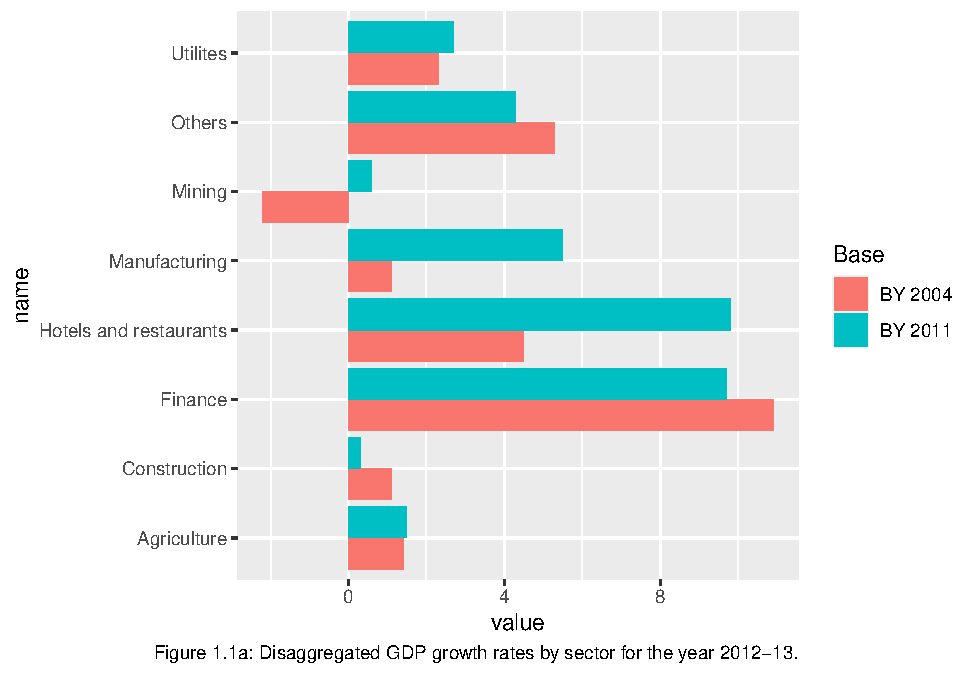
\includegraphics{thesis_files/figure-latex/unnamed-chunk-3-1} \end{center}
 \begin{center}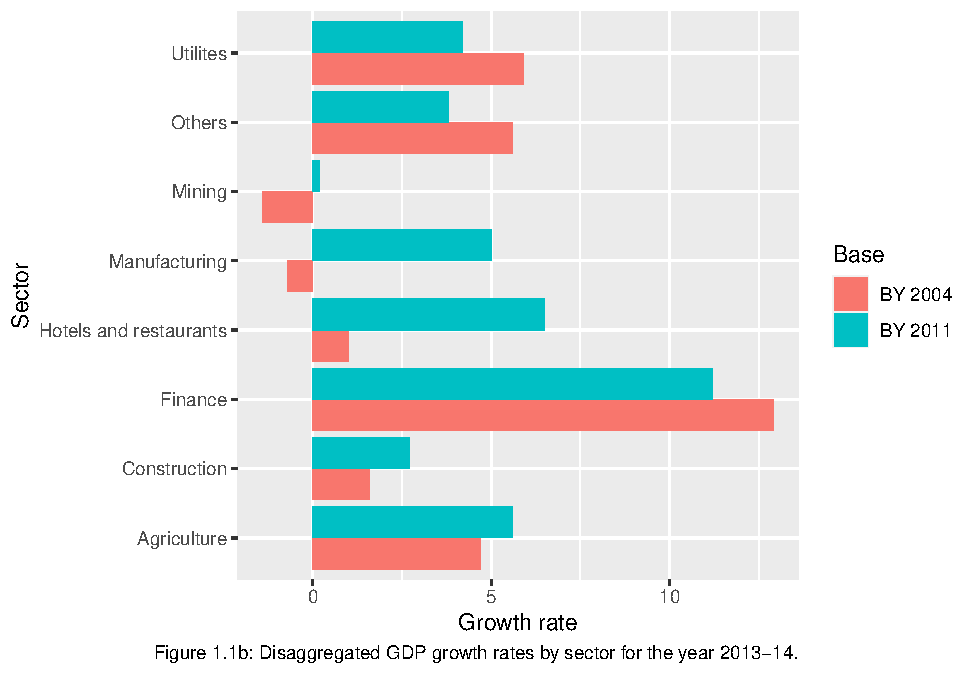
\includegraphics{thesis_files/figure-latex/unnamed-chunk-3-2} \end{center}

 \hypertarget{conclusion}{%
 \section{Conclusion}\label{conclusion}}

 \hypertarget{the-synthetic-control-method}{%
 \chapter{The Synthetic Control Method}\label{the-synthetic-control-method}}

 The synthetic control method is a relatively recent innovation in causal inference. It was first introduced by Alberto Abadie and Javier Gardeabazal in their 2003 paper investigating estimating the impact of conflict on GDP in the Baque county (\protect\hyperlink{ref-abadie_economic_2003}{Abadie \& Gardeazabal, 2003}). Since then, the method has been used widely to study the impact of policy interventions involving large economic units like cities, states or countries (\protect\hyperlink{ref-abadie_synthetic_2010}{Abadie, Diamond, \& Hainmueller, 2010}, \protect\hyperlink{ref-abadie_comparative_2015}{2015}). Nobel laureate Guido Imbens and Susan Athey call it ``arguably the most important innovation in the policy evaluation literature in the last 15 years'' in a recent review of applied econometrics (\protect\hyperlink{ref-athey_state_2017}{Athey \& Imbens, 2017}).
 \linebreak

 In this chapter, I present an overview of the synthetic control method (SCM), beginning with a non-technical introduction. In Section 2.2, I examine the theory behind the method, focussing on the setup, estimation and inference. In Section 2.3, I present the advantages and limitations of the SCM. I review the advances in the literature on alternative estimation methods in Section 2.4. In Section 2.5 I delve deeper into the mechanics of the generalized synthetic control methods (GSCM) and conclude in the last sectiomn

 \hypertarget{introduction}{%
 \section{Introduction}\label{introduction}}

 Synthetic control methods emerged in the context of comparative case studies. Case studies often study the effect of a policy or intervention on a particular outcome, by comparing it to other determinants of the outcome. For example, a medicine case study focuses on an ailment, while a political case study examines the impact of an electoral strategy. Comparative case studies compare one or more units exposed to the event or intervention of interest to one or more unexposed units. For example, Abadie et al. (\protect\hyperlink{ref-abadie_synthetic_2010}{2010}) examines the impact of Proposition 99, a tobacco control program implemented in California and compares its impact on cigarette sales relative to other states. Only some units must be exposed to the intervention, while other comparable units are not.
 \linebreak

 Comparative case studies have been used in economics for a long time. However, studies typically relied on the comparison between one unit where a policy was implemented (also called `treatment' unit) to a similar unit, where the policy did not take place (also called `control' unit). A classic example is the study by Card (\protect\hyperlink{ref-card_impact_1990}{1990}). Card examines the impact of the Mariel boatlift, which bought Cuban workers to Miami on the wages of low-skilled workers. He considers various single `control' cities like Houston or Philadelphia, where no such event took place to estimate the difference between wages. The key assumption here is that wages in Miami and the control city would be the same, had the boatlift not taken place. This method is the classic difference-in-difference approach, which has been since used widely in economics(\protect\hyperlink{ref-card_minimum_1994}{Card \& Krueger, 1994}; \protect\hyperlink{ref-dube_minimum_2010}{Dube, Lester, \& Reich, 2010}), with interesting updates to the original methodology(\protect\hyperlink{ref-goodman-bacon_difference-differences_2021}{\textbf{goodman-bacon\_difference-differences\_2021?}}; \protect\hyperlink{ref-callaway_difference-differences_2021}{\textbf{callaway\_difference-differences\_2021?}}).
 \linebreak

 Synthetic control builds upon difference-in-differences, with the key difference being that instead of considering a single control, a weighted average of a group of controls is considered. When the control group is small in number, their weighted average provides a better unit of comparison than any single entity(\protect\hyperlink{ref-abadie_using_2021}{Abadie, 2021}). Specifically, the estimator chooses the weights such that this combination of control units reflects the treated unit closely. This is the approach followed in Abadie et al. (\protect\hyperlink{ref-abadie_synthetic_2010}{2010}). The authors use a weighted average of cigarette sales, composed of 38 states, to study the impact of Proposition 99 in California.
 \begin{figure}

 {\centering 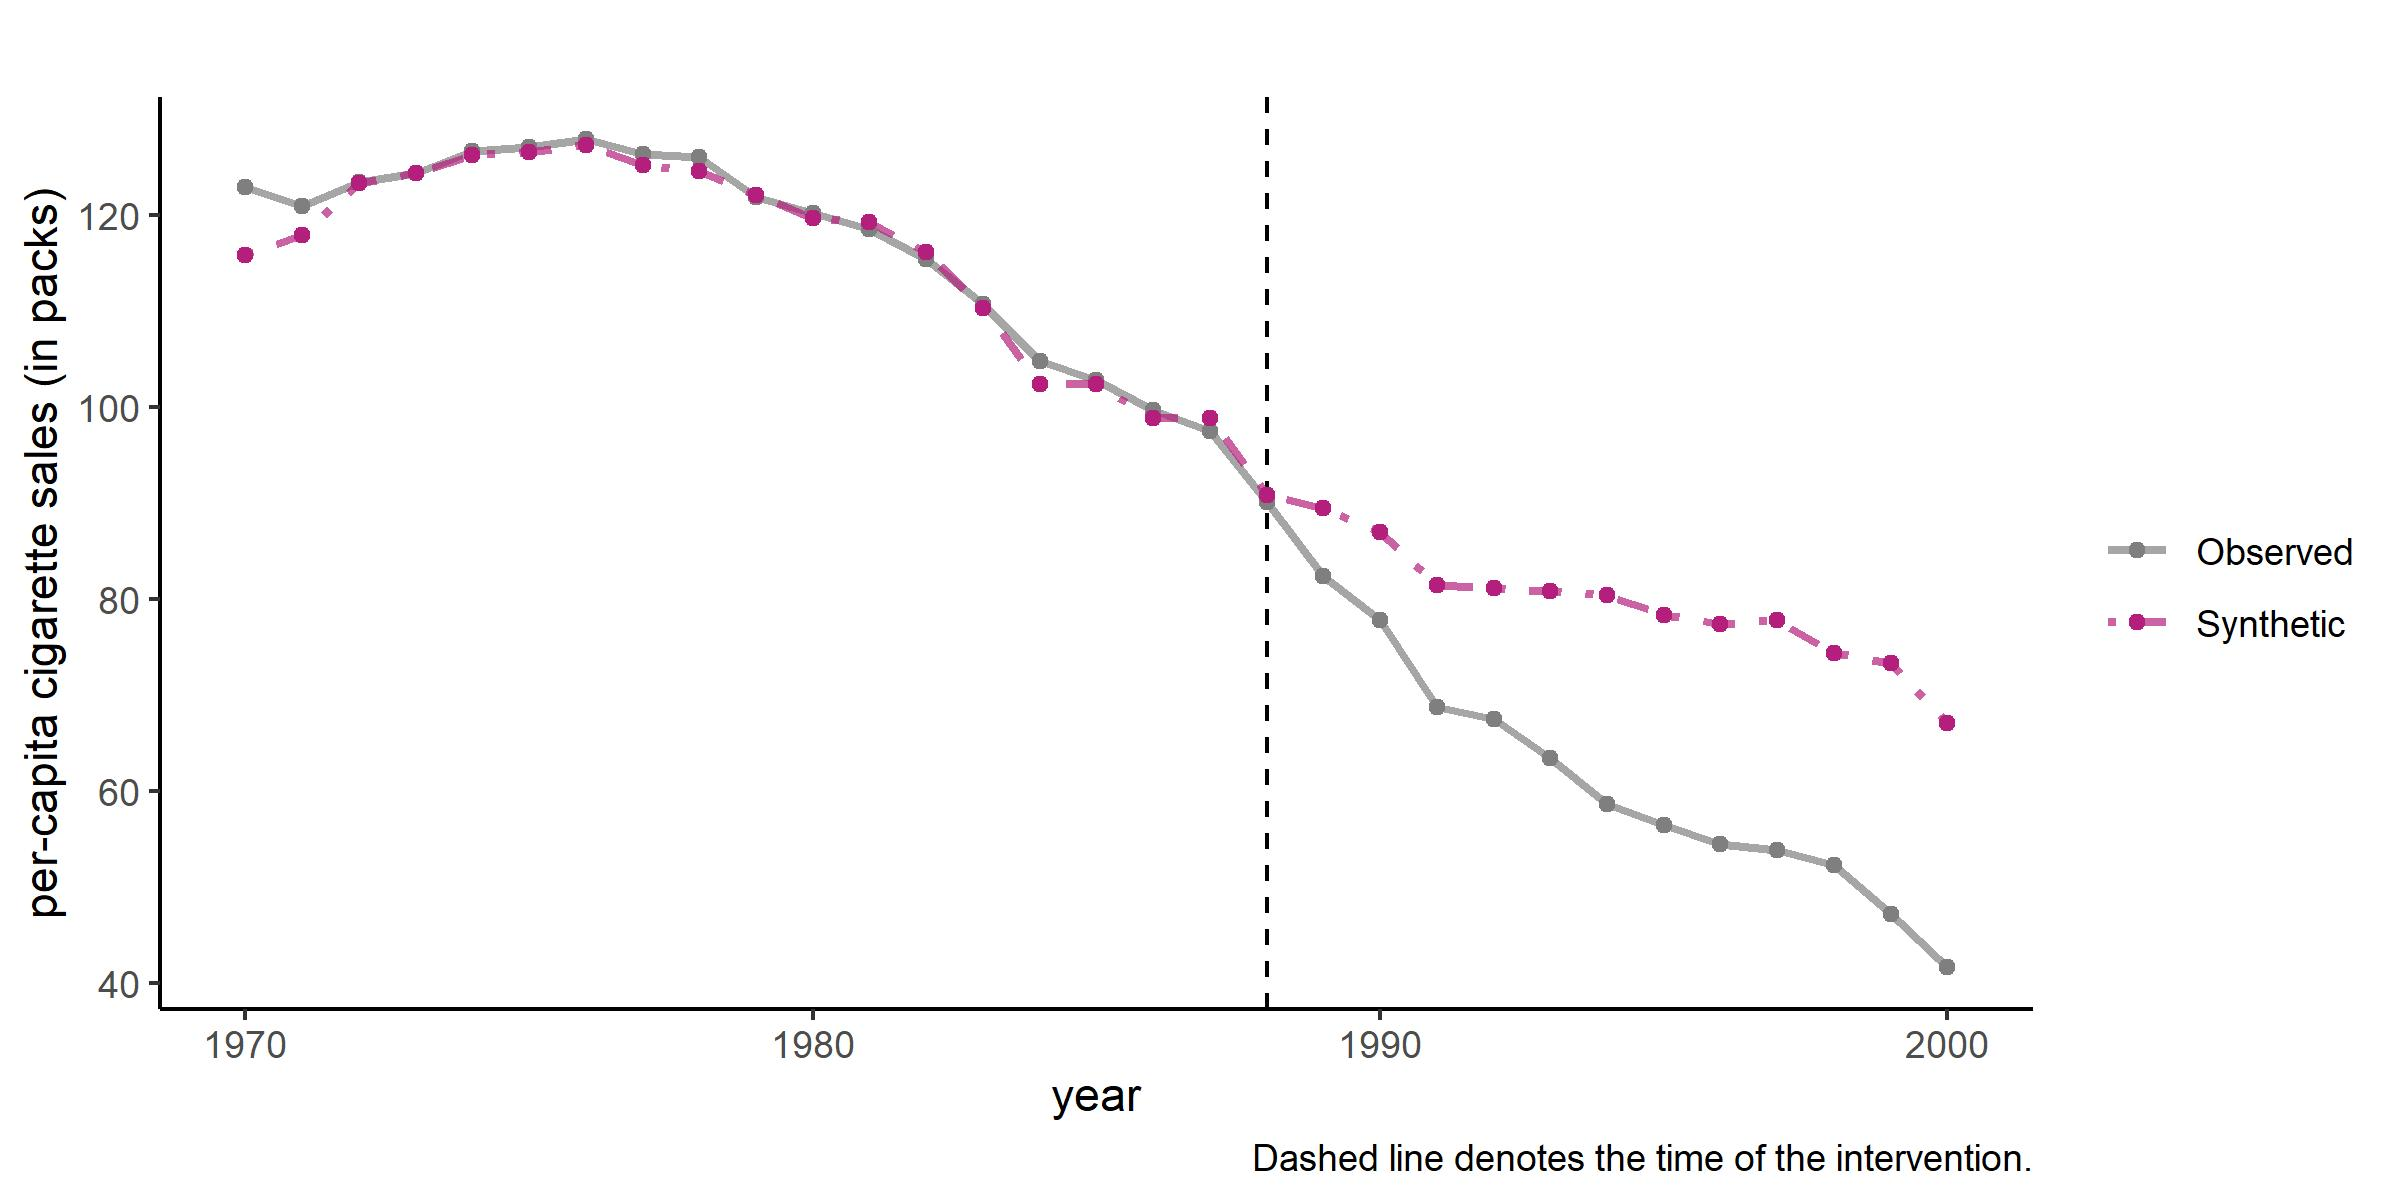
\includegraphics[width=1\linewidth]{figure/caltrends} 

 }

 \caption{Synthetic Control of Californoa}\label{fig:prop}
 \end{figure}
 Figure \ref{fig:prop} shows the per capita cigarette sales in California and synthetic California from 1970-2000. According to the SCM model, synthetic California is an estimation of what cigarette sales in California would have been, had Proposition 99 not existed. The gap between the two trends post the treatment year (1988), shows that cigarette sales would have been significantly higher in the counterfactual, indicating that the law was successful in reducing tobacco consumption in California. Thus, the SCM offers a very clean and intuitive way to estimate the causal effect of a policy intervention with a small number of large units, like cities, counties or countries. In the next section, I introduce the formal model and elaborate on how estimation and inference take place.

 \hypertarget{formal-aspects}{%
 \section{Formal Aspects}\label{formal-aspects}}

 To maintain consistency of notation, I stick to the model setup as seen in Abadie (\protect\hyperlink{ref-abadie_using_2021}{2021}).

 \hypertarget{setup}{%
 \subsection{Setup}\label{setup}}

 We begin by observing data for \(J+1\) units, where \(j=1,2,...,J+1\). Assume that \(j=1\) is the first unit is the unit where the intervention occurred or the treated unit. The rest of the units, from \(j=2,3...J+1\), form the set of units unaffected by the treatment and are referred to as the donor pool. Let the data be observed for \(T\) periods, where the first \(T0\) periods are those before the intervention. The outcome of interest observed for unit \(j\) at time \(t\) is referred to as \(Y_{jt}\). We also observe \(k\) predictors of the outcome \(j\), \(X_{1j}......X_{kj}\). The vectors \(\mathbf{X_{1},…,X_{j+1}}\) contain the values of the predictors for units \(j = 1,…,J + 1\), respectively. The \(k \times J\) matrix, \(\mathbf{X0} = [\mathbf{X2},..., \mathbf{XJ+1}]\), collects the values of the predictors for the J untreated units.
 \linebreak

 For unit \(j\) in time \(t\), the potential response \emph{without} the intervention is defined as \(Y^{N}_{jt}\), while for the unit affected by the intervention \(j=1\) at time \(t>T0\), the potential response is defined as \(Y^{I}_{1t}\). Thus the effect of the intervention at \(t>T0\) is given by

 \[\alpha_{1t}= Y^{I}_{1t}-Y^{N}_{jt}\]
 Since the unit of interest is observed after \(T0\), we have \(Y_{1t}=Y^{I}_{1t}\). The unknown response is the counterfactual, which is the evolution of the outcome of interest in absence of the intervention for \(t>T0\). Now, let \(D_{it}\) take the value 1 if unit \(i\) is exposed to the intervention and 0 otherwise. Then the observed outcome \(Y_{it}\) is given by
 \begin{equation}
 Y_{it}= Y^{N}_{it} + \alpha_{it} D_{it}
 \label{eq:eq1}
 \end{equation}
 As only the first unit is exposed to the treatment and only after \(T0\), we have
 \begin{equation}
 D_{it} = 
 \begin{cases} 
 1 & \text{if} i=1, t>T0 \\
  0 &\text{otherwise}
 \end{cases}
 \label{eq:eq2}
 \end{equation}
 The effect of intervention on unit 1 at time \(t>T0\), given by \(alpha_{1t}\), is
 \begin{equation}
 \alpha_{1t}= Y^{I}_{1t}-Y^{N}_{1t}= Y_{1t}-Y^{N}_{1t}
 \label{eq:eq3}
 \end{equation}
 Since \(Y_{1t}\) is observed after the intervention, we simply need to estimate \(Y^{N}_{1t}\) to estimate \(\alpha_{1t}\).

 \hypertarget{estimation}{%
 \subsection{Estimation}\label{estimation}}

 Assume that \(Y^{N}_{1t}\) is given by a linear factor model. Initially used as a model of psychological evaluations (\protect\hyperlink{ref-spearman_general_1904}{Spearman, 1904}), linear factor models are used to model unobserved heterogeneity in economics. Typically, the idiosyncratic error term has a defined structure, consisting of a limited number of unobserved common factors, and their parameters, known as factor loadings. The model used to estimate SC is given by
 \begin{equation}
 Y^{N}_{1t}= \delta_{t}+\mathbf{\theta_{t} Z_{i}}+\mathbf{\lambda_{t} \mu_{i}}+ \epsilon_{it}
 \label{eq:eq4}
 \end{equation}
 where \(\delta_{t}\) is the time trend, \(\mathbf{Z_{i}}\) is a vector of observed covariates not affected by the intervention and \(\mathbf{ \lambda_{t}}\) is a vector of unobserved common factors. \(\mathbf{\theta_{t}}\) and \(\mathbf{\mu_{i}}\) are vectors of unknown parameters and unknown factor loadings respectively. \(\epsilon_{it}\) is the zero-mean error term. Now, consider a \((j\times 1)\) vector of weights \(\mathbf{W}=(w_{2},..,w_{j+1})\), where each weight is positive and the sum of weights equals one. Thus, the weighted value of the outcome variable is
 \begin{equation}
 \sum_{j=2}^{J+1}w_{j}Y^{N}_{jt}= \delta_{t}+
 \mathbf{\theta_{t}} \sum_{j=2}^{J+1}w_{j}\mathbf{Z_{j}}+
 \mathbf{\lambda_{t}} \sum_{j=2}^{J+1}w_{j}\mathbf{\mu_{j}}+ \sum_{j=2}^{J+1}w_{j}\epsilon_{jt}
 \label{eq:eq5}
 \end{equation}
 Suppose there exist a set of optimal weights \((w_{2}^{*},...,w_{j}^{*})\), such that,

 \[\sum_{j=2}^{J+1}w_{j}^{*}Y_{j1}=Y_{11}\]

 \[ \sum_{j=2}^{J+1}w_{j}^{*}Y_{j2}=Y_{12}\]

 \[\sum_{j=2}^{J+1}w_{j}^{*}Y_{jT0}=Y_{1T0} \]

 \[\sum_{j=2}^{J+1}w_{j}^{*} \mathbf{Z_{j}}=\mathbf{Z_{1}}\]

 These set of weights \((w_{2}^{*},...,w_{j}^{*})\) are such that the weighted sum of each observed outcome variable for the donor group, in the pre-intervention period \(T0\) (\(Y_{j1},..., Y_{jT0}\)) equals the respective outcome variable for the treated unit before the intervention (\(Y_{11},...,Y_{1T0}\)). Similarly, the weighted sum of donor group covariates equals the covariates for the treated unit. In the Proposition 99 example, all the variables on the right-hand side would be the observed per capita cigarette sales in California before 1988, while the terms on the left-hand side denote the weighted sum of per capita cigarette sales in the donor states. From Equation \eqref{eq:eq4}, we have
 \begin{equation}
 \hat{Y^{N}_{1t}}=\sum_{j=2}^{J+1}w_{j}Y^{N}_{jt}
 \label{eq:eq6}
 \end{equation}
 and
 \begin{equation}
 \hat{\alpha_{1t}}={Y_{1t}}-\hat{Y^{N}_{1t}}
 \label{eq:eq7}
 \end{equation}
 Equation \eqref{eq:eq6} states that the estimated synthetic control for the unobserved outcome is given by the weighted average of the observed outcome variables in the donor group. This is true as each observation of the estimated synthetic control (\textbackslash hat\{Y\^{}\{N\}\_\{1t\}) is the weighted average of each observation in the donor group (Equations 6-10). Once the synthetic control is estimated, the treatment effect for the affected unit is simply the difference between the observed outcome and the estimated unobserved outcome in \(t>T0\), as shown in Equation \eqref{eq:eq7}.
 \linebreak

 How are the optimal weights determined? Abadie et al. (\protect\hyperlink{ref-abadie_synthetic_2010}{2010}) argue that the weights should be chosen so that the synthetic control best resembles the pre-treatment values of the predictors of the outcome variable. As stated before, \(\mathbf{X1}\) contains the pre-treatment values of the covariates which predict the outcome variable for the treated unit, while \(\mathbf{X0}\) refers to the same for the donor units. Then, the vector of weights \(\mathbf{W^*}\), minimizes

 \[||\mathbf{X1}-\mathbf{X0 W}||=\sqrt{(\mathbf{X1}-\mathbf{X0 W})' \mathbf{V} (\mathbf{X1}-\mathbf{X0 W})}\]
 The matrix \(\mathbf{V}\) measures the discrepancy between the\(\mathbf{X1}\) and \(\mathbf{X0}\). The choice of \(\mathbf{V}\) is an important one and influences the quality of the pre-intervention fit. Abadie et al. (\protect\hyperlink{ref-abadie_synthetic_2010}{2010}) chooses \(\mathbf{V}\), such that the synthetic control minimizes the mean squared prediction error (MSPE)

 \[ \sum_{t \in T0}(Y_{1t}- w_{2}(\mathbf{V})Y_2{t}-...-w_{J+1}(\mathbf{V})Y_{J+1t})^2\]
 The MSPE is a measure of the distance between the outcome variable of the treated unit (\(Y_{1t}\)) and the predicted outcome variable generated by the synthetic control. It is crucial to infer the outcome of the synthetic control, which is explained in the next section.

 \hypertarget{inference}{%
 \subsection{Inference}\label{inference}}

 At a preliminary level, inference can be done using placebo tests. Placebo tests apply the synthetic control tests to each of the donor units i.e.~the units where the intervention does not occur. If the gap between the observed and synthetic values is of a magnitude similar to those seen in the unit of interest, then there is no significant evidence that the intervention had the desired effect. However, if the magnitudes are smaller, then it can be concluded that the intervention did have a significant effect on the unit of interest.
 \begin{figure}

 {\centering 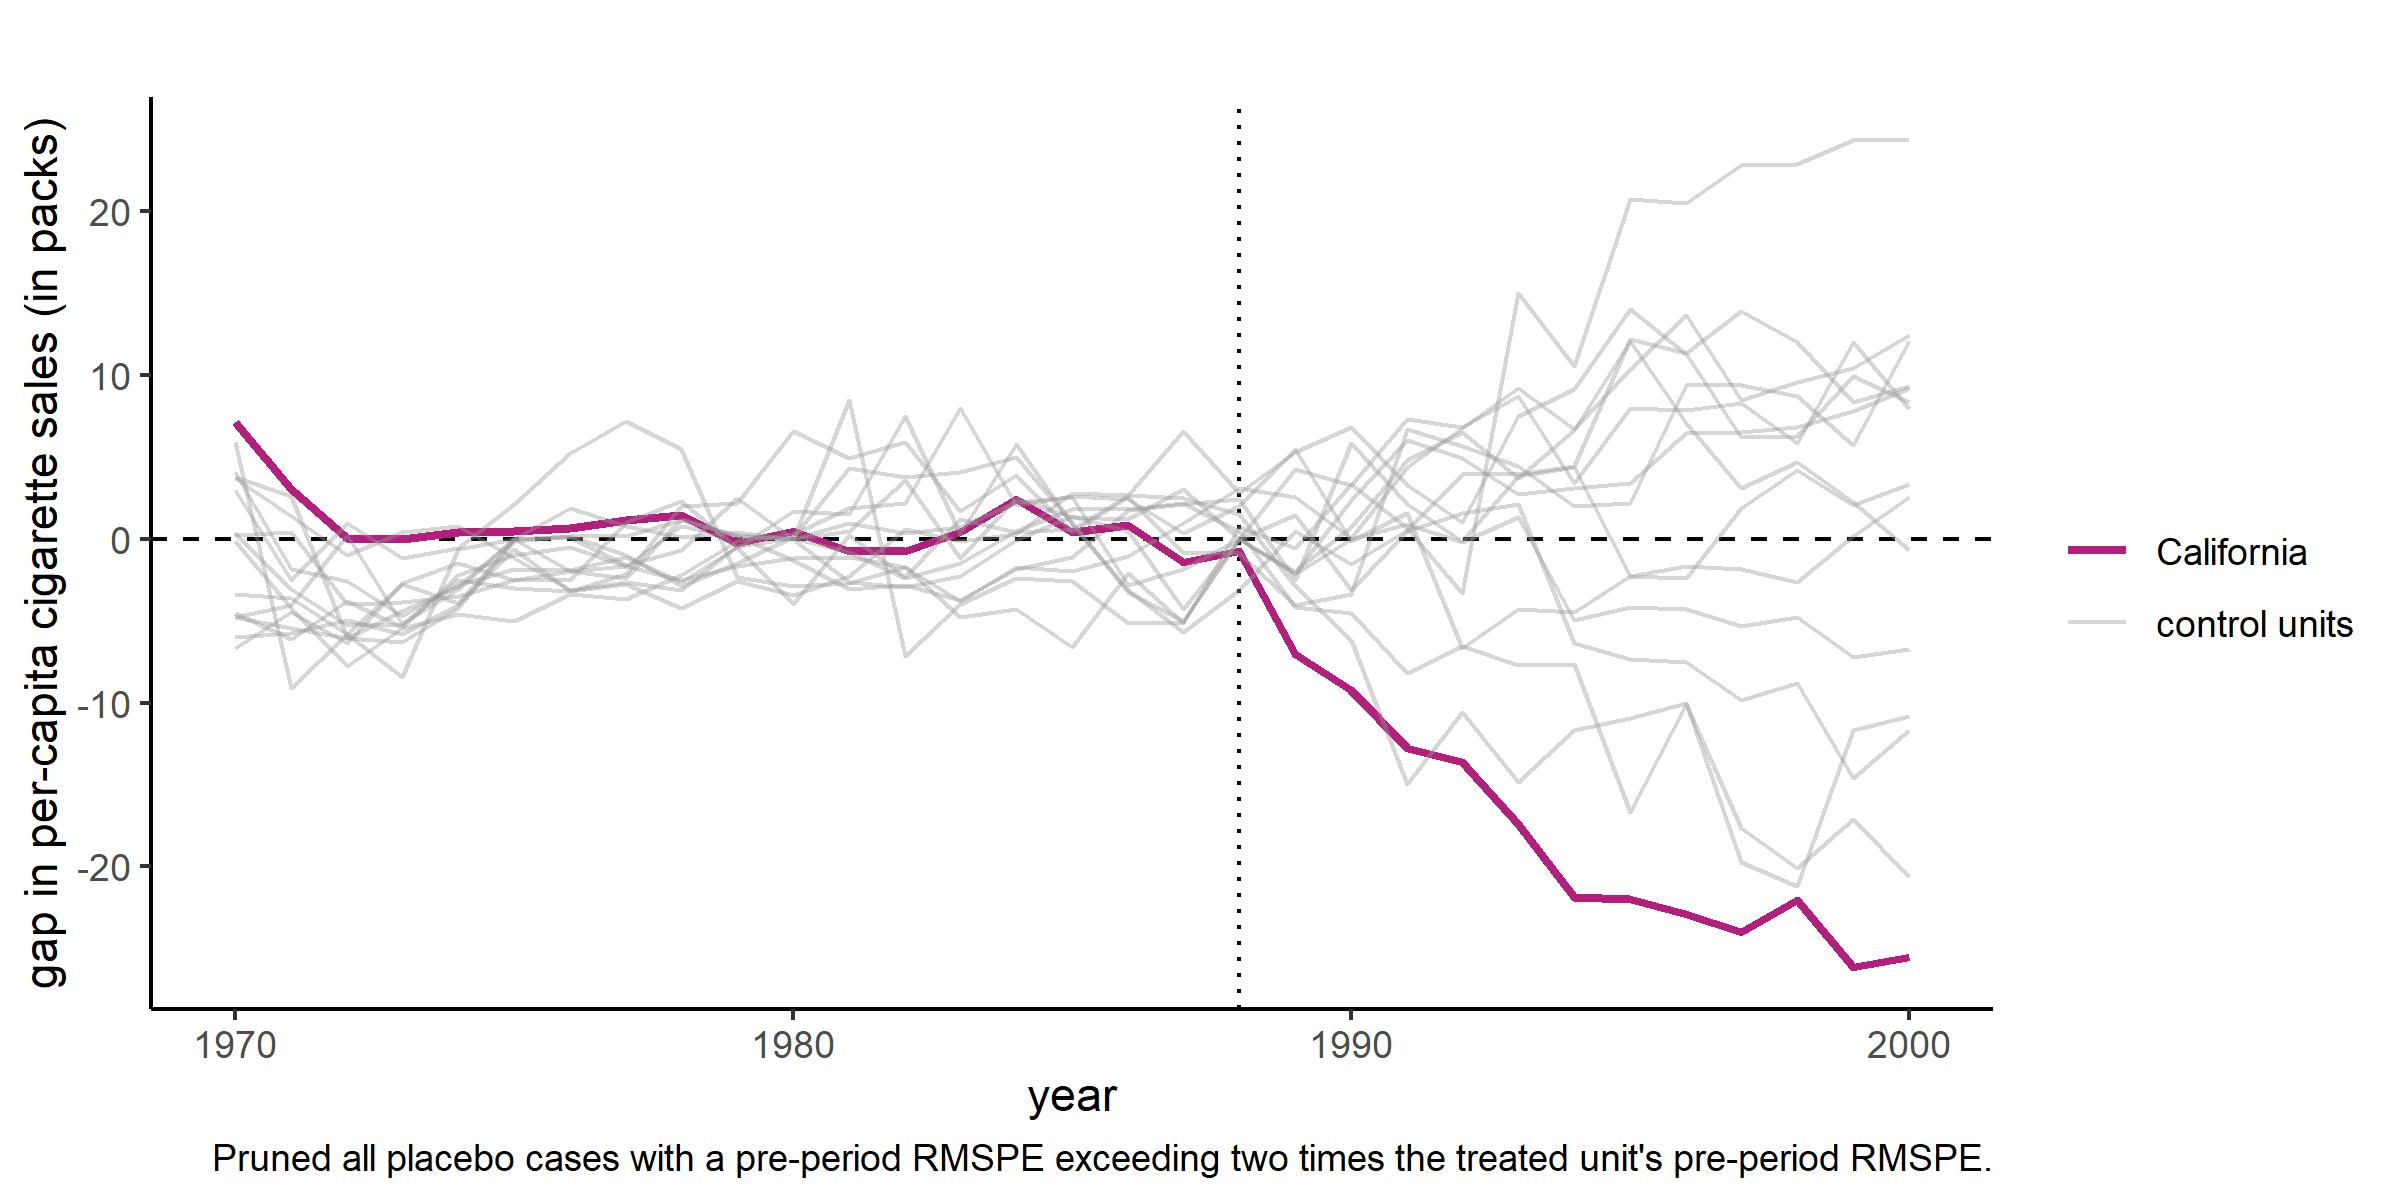
\includegraphics[width=1\linewidth]{figure/calplacebo} 

 }

 \caption{Per-capita cigarette sales gaps in California and placebo gaps in 19 control states}\label{fig:placebo}
 \end{figure}
 Figure \ref{fig:placebo} shows the gap in the per capita cigarette sales in the placebo states as well as California. The cigarette sale gap is highest in the state of California, showing that the effect of Proposition 99 was significant in size. The sample is restricted to 19 states, as units with a pre-intervention MSPE greater than 2 times that of California are discarded. This is done to exclude states which are too similar to California.
 \linebreak

 While being a useful starting point, placebo tests are limited as the pre-treatment fit of all the placebo units may not closely match the trajectory of the outcome variable well. For this reason, Abadie et al. (\protect\hyperlink{ref-abadie_synthetic_2010}{2010}) specifies an exact test statistic, which measures the ratio of the post-intervention fit relative to the pre-intervention fit. This is given by
 \begin{equation}
 r_{j}= \frac{R_{j}(T_{0}+1,T)}{R_{j}(1,T_{0})}
 \label{eq:eq8}
 \end{equation}
 where
 \begin{equation}
 R_{j}(t_{1},t_{2})= (\frac{1}{t_{2}-t_{1}+1} \sum_{t=t1}^{t2}(Y_{jt}-Y_{jt}^{N})^2)^{\frac{1}{2}}
 \label{eq:eq9}
 \end{equation}
 Equation \eqref{eq:eq9} defines the mean squared prediction error (MSPE) of the synthetic control estimator over periods \(t_{1}\) to \(t_{2}\). Hence, the numerator of Equation \eqref{eq:eq8} is the MSPE of the post-intervention period, and the denominator is the MSPE of the pre-intervention period. The p-value for this inferential procedure is given by:
 \begin{equation}
 p= (\frac{1}{J+1} \sum_{j=1}^{J+1}I_{+}(r_{j}-r_{1})
 \label{eq:eq10}
 \end{equation}
 where \(I_{+}(.)\) is an indicator function taking value one for non-negative inputs and zero otherwise.
 \begin{figure}

 {\centering 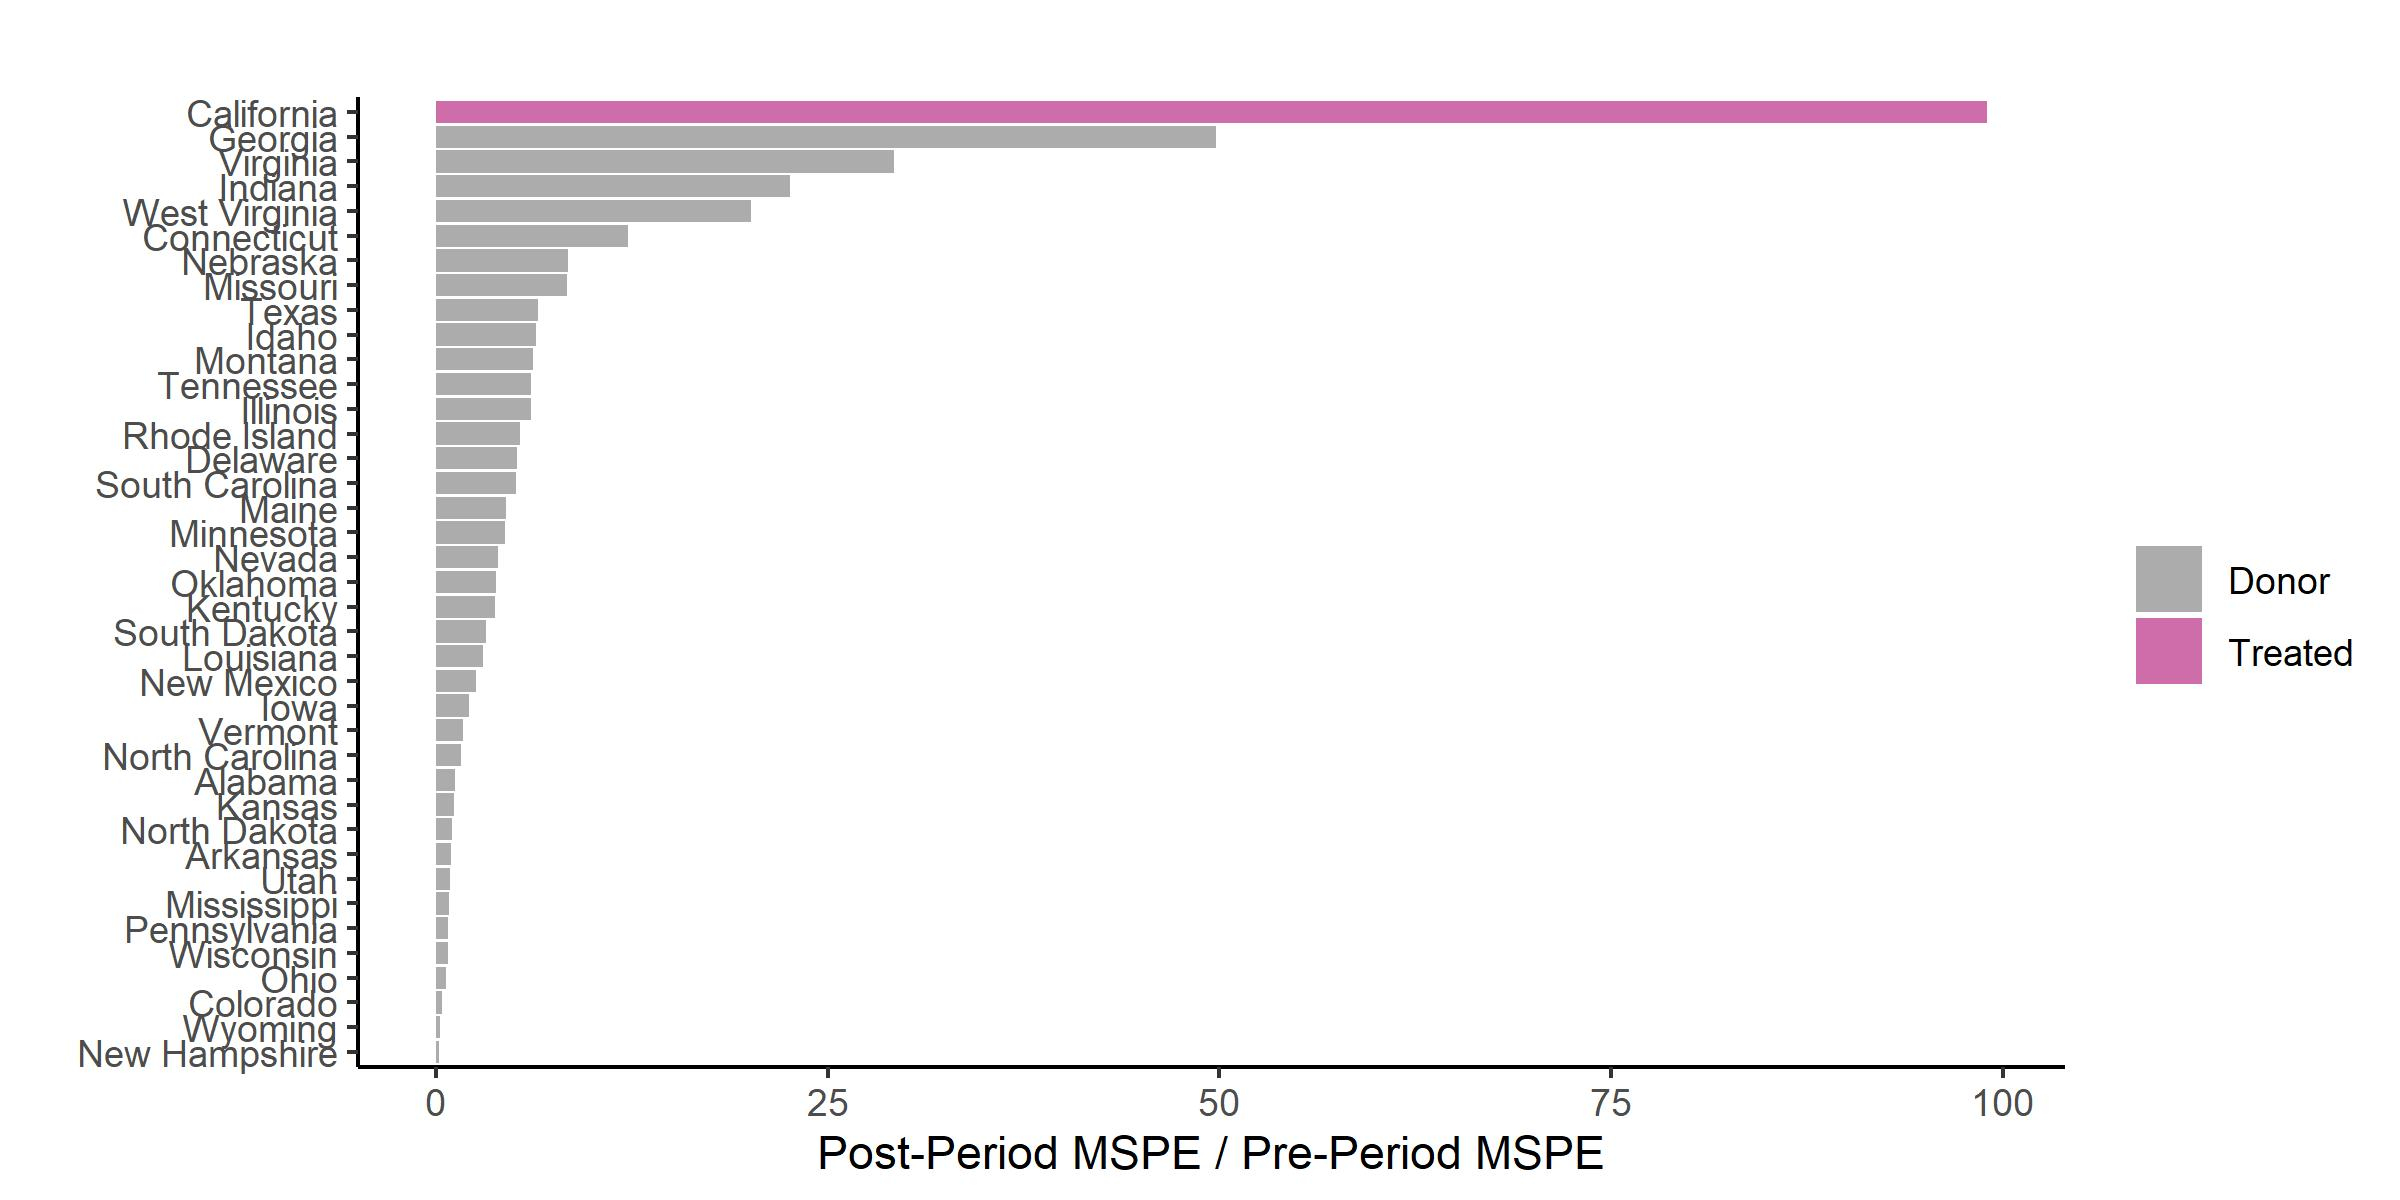
\includegraphics[width=1\linewidth]{figure/calmspe} 

 }

 \caption{Ratio of post and pre-treatment MSPE in California and donor states}\label{fig:mspe}
 \end{figure}
 To better understand how to interpret this test statistic, consider again the Proposition 99 example. Figure \ref{fig:mspe} shows the value of the test statistic, i.e.~the ratio of the post-treatment to the pre-treatment MSPE for the treated state (California) and each of the states belonging to the donor pool. The MSPE is the squared value of the absolute distance between the fitted cigarette sales and actual cigarette sales. If Proposition 99 had a significant effect on cigarette sales in California, then the pre-treatment trend of California and synthetic California overlap, and diverge in the post-treatment period. Hence, the ratio of the two MSPEs should be the largest for California, which is exactly what is seen in Figure \ref{fig:mspe}. Furthermore, using equation \eqref{eq:eq10} the corresponding p-values of this statistic can be computed, as shown in Table 2.1.
 \begin{table}[h!!]
 \centering
 \begin{tabular}{llr}
 \hline
 \hline
 \textbf{Unit name} & \textbf{Type}&\textbf{p-values}\\
 \hline
 \hline
 California & Treated & 0.0256410\\
 \hline
 Georgia & Donor & 0.0512821\\
 \hline
 Virginia & Donor & 0.0769231\\
 \hline
 Indiana & Donor & 0.1025641\\
 \hline
 West Virginia & Donor & 0.1282051\\
 \hline
 Connecticut & Donor & 0.1538462\\
 \hline
 Nebraska & Donor & 0.1794872\\
 \hline
 Missouri & Donor & 0.2051282\\
 \hline
 Texas & Donor & 0.2307692\\
 \hline
 Idaho & Donor & 0.2564103\\
 \hline
 \end{tabular}
 \label{tab:tab1}
 \caption{p-values for the Post-Pre Intervention MSPE Ratio for select states}
 \end{table}
 The p-value for California is about 2.5\%, making the test statistic significant at 5\%.

 \hypertarget{advantages-and-limitations-of-scm}{%
 \section{Advantages and Limitations of SCM}\label{advantages-and-limitations-of-scm}}

 The standard synthetic control method, estimated as per Abadie et al. (\protect\hyperlink{ref-abadie_synthetic_2010}{2010}) has several advantages. The first distinct advantage of the standard SCM is that it gives a transparent fit. Specifically, the discrepancy between the treated unit and the combination of the donor units can be seen clearly. This can be done by computing the difference between the pre-treatment averages of the variables of interest for the treated unit and the corresponding synthetic control. In continuation, the weights assigned to each of the donor units are also easily accessible, which allows the researcher to understand which units are more similar to the treated unit, and which are not. Secondly, synthetic control methods preclude extrapolation due to the constraint that the sum of the weights is one. A regression model, in contrast, allows for negative weights. Finally, SCM provides a safeguard against `specification searches', which means cherry-picking models which yield a known result. This is avoided in SCM, as all the information used to compute the estimator is taken from the pre-intervention period, while the counterfactual for the post-intervention period remains unknown. Finally, SCM results are geometrically intuitive and can be easily visualized, and interpreted through placebo and exact test statistics.
 \linebreak

 However, the standard SCM has some limitations, two of which I highlight here. The first, elaborated by Ferman, Pinto, \& Possebom (\protect\hyperlink{ref-ferman_cherry_2020}{2020}), relates to specification searching opportunities. The choice of contributors to the synthetic control is often a matter of discretion, and hence it is possible to try and test several combinations which yield a desired pre-treatment fit and post-treatment trend. There is significant room for such searches when the number of pre-treatment periods is close to those used in common applications. While the distance function is minimized algorithmically, which limits the bias, the function itself is endogenously chosen by the researcher, creating the potential for bias and ``p-hacking''(\protect\hyperlink{ref-cunningham_causal_2021}{Cunningham, 2021}).
 \linebreak

 Another common critique centres on the restriction placed on weights: that they must be positive and sum up to one. In technical terms, this is the ``convex hull assumption'', wherein the weighted average (or convex combination) of the predictors of the donor pool falls close to the convex hull of these points. This restriction leads to sparse distribution of weights, with a small number of units contributing heavily to the synthetic control, and many units contributing close to zero. Since there are typically multiple predictors, and they are to be determined such that the synthetic control resembles the treated unit both in terms of the outcome and the predictors, the weights of the predictors are the control units are jointly optimized. However, multiple studies have shown that the weights produced by algorithms using such joint optimization procedures are unstable and sub-optimal (\protect\hyperlink{ref-becker_estimating_2017}{Becker \& Klößner, 2017}; \protect\hyperlink{ref-klosner_comparative_2018}{Klößner, Kaul, Pfeifer, \& Schieler, 2018}). Kuosmanen, Zhou, Eskelinen, \& Malo (\protect\hyperlink{ref-kuosmanen_design_2021}{2021}) use insights from game theory to show that the true optimum of this estimation procedure is a corner solution, which assigns all the weight to a single predictor, which defeats the purpose of the SCM. These limitations, along with some others (not discussed here) have led to the development of alternatives to the SCM.

 \hypertarget{alternative-estimators}{%
 \section{Alternative Estimators}\label{alternative-estimators}}

 Since its introduction in Abadie \& Gardeazabal (\protect\hyperlink{ref-abadie_economic_2003}{2003}), the synthetic control method has become a popular tool of causal inference. However, it has also been criticised for reasons mentioned in the previous section; the critiques have also spawned many alternatives. Some of these are improvements to the standard SCM, while others use different estimation techniques altogether. Ferman \& Pinto (\protect\hyperlink{ref-ferman_synthetic_2021}{2021}) deals with the issue of imperfect pre-treatment fit. When the matching of pre-treatment predictors of the treated and the donor units is imperfect, the SCM estimator is biased, even for a large pre-treatment period. However, using a demeaned version of the SCM reduces the bias of the estimator relative to difference-in-differences. Ben-Michael, Feller, \& Rothstein (\protect\hyperlink{ref-ben-michael_augmented_2021}{2021}) also deals with the issue of bias but instead proposes a bias correction by modifying the regression specification, called the augmented SCM. The predictor matching discrepancy is corrected in this case, by using a ``penalty term'', which is a synthetic control estimator applied to residuals. Extrapolation is penalized with a ridge-linear model, which improves pre-treatment fit. The SCM can also be extended to include multiple treated units, which leads to a multiplicity of possible solutions and more scope for matching discrepancy. Abadie \& L'Hour (\protect\hyperlink{ref-abadie_penalized_2021}{2021}) proposes a penalizer for pairwise discrepancies between treated and control units, in a multiple unit setup.
 \linebreak

 A subset of the literature uses matrix completion methods for SCM estimation. This involves assuming a nonlinear factor model for the untreated units, allowing for missing values, which are then estimated using matrix completion methods. Linear combinations of the estimated matrix are then used to construct the synthetic controls. This can be done in a setup without covariates (\protect\hyperlink{ref-amjad_robust_2018}{Amjad, Shah, \& Shen, 2018}), and with covariates (\protect\hyperlink{ref-amjad_mrsc_2019}{Amjad, Misra, Shah, \& Shen, 2019}). Athey, Bayati, Doudchenko, Imbens, \& Khosravi (\protect\hyperlink{ref-athey_matrix_2021}{2021}) assume that the untreated units are composed of a matrix and a random error term, and the matrix values are estimated using completion techniques. Their methodology allows for the inclusion of covariates and various fixed effects. Some other papers allow for regression-based weights and extrapolation. Doudchenko \& Imbens (\protect\hyperlink{ref-doudchenko_balancing_2016}{2016}) allow for negative weights that may not sum up to one, where the weights are regularized using an elastic net (a combination of lasso and ridge) to impose penalties. The augmented SCM also allows negative weights, as does the Generalized SCM (\protect\hyperlink{ref-xu_generalized_2017}{Xu, 2017}). Arkhangelsky, Athey, Hirshberg, Imbens, \& Wager (\protect\hyperlink{ref-arkhangelsky_synthetic_2021}{2021}) introduces an estimator that includes not only control unit weights but also pre-intervention time weights, called the synthetic difference-in-difference estimator.
 \linebreak

 Finally, studies have proposed alternatives to the inference procedure adopted by Abadie et al. (\protect\hyperlink{ref-abadie_synthetic_2010}{2010}), which uses a permutation test (the SC is calculated by considering every possible control unit). Hahn \& Shi (\protect\hyperlink{ref-hahn_synthetic_2017}{2017}) show that for the placebo tests to be valid the symmetry assumption must hold i.e.~the distribution of the difference between the pre-treatment outcome variable and the estimated synthetic control must be identical. The authors show that this may not always hold for the standard SCM and propose using the following test: comparing the value of treatment effects of \(T-T_{0}\) post-intervention periods to the distribution of the same values computed for every subset for that number of periods. Chernozhukov, Wüthrich, \& Zhu (\protect\hyperlink{ref-chernozhukov_exact_2021}{2021}) suggests a conformal inference procedure, starting by assuming that the counterfactual is composed of a mean unbiased proxy and an error term. With the pre and post-intervention outcomes differing only by the treatment effect, the distribution of a function of the post-intervention error terms should be the same as that of a random permutation of the same. In the case of the SCM, this can be tested by setting the proxy as the synthetic control and implementing the test on the residuals computed via least squares. Chernozhukov, Wuthrich, \& Zhu (\protect\hyperlink{ref-chernozhukov_t-test_2021}{2021}) provides a methodology for computing an exact t-test for the SC estimator.
 \linebreak

 The literature on the synthetic control method is thus rich and developing fast. For the remained of the chapter, I delve deeper into the generalized synthetic control method, which includes many of the advances in the literature - specifically, the inclusion of multiple treated units, regression-based weights, and robust inference procedures.

 \hypertarget{generalized-synthetic-control}{%
 \section{Generalized Synthetic Control}\label{generalized-synthetic-control}}

 The generalized synthetic control was proposed by Yiqing Xu in 2017. This method combines the synthetic control method and the interactive fixed effects model (IFE). The IFE model, proposed by Bai (\protect\hyperlink{ref-bai_panel_2009}{2009}), is used to model unobserved time-varying confounders. Time-varying confounders refer to unobserved variables that are correlated with both the dependent and independent variables, and which take different values over time. The IFE model interacts unit-specific intercepts, referred to as factor loadings and time-varying coefficients, referred to as latent factors. The generalized synthetic control method (GSCM), unifies the IFE model with the SCM in the following way: first, using only the control group (or donor pool) data, it estimates an IFE model to obtain a fixed number of latent factors. Then, the factor loadings for each treated unit are estimated by linearly projecting pre-treated treated outcomes on the space spanned by this factor. Finally, it computes treated counterfactuals based on the latent factors and the factor loadings.
 \linebreak

 The key difference between the SCM and GSCM is that the latter does dimension reduction before re-weighting. Specifically, the model selects the number of latent factors to be used algorithmically. This is done using a cross-validation scheme (details in the inference section), which avoids specification searches. The GSCM is also more ``general'' in the sense that it can be extended to cases with multiple treated units and variable treatment periods.

 \hypertarget{framework}{%
 \subsection{Framework}\label{framework}}

 In this section and the next one, I stick to the notation used in Xu (\protect\hyperlink{ref-xu_generalized_2017}{2017}). Let \(Y_{it}\) be the outcome of interest for unit \(i\) and time \(t\), and let \(O\) and \(C\) denote the total number of units in the treatment and control groups, with \(N\) total units. All units are observed for \(T\) periods, with the pre-treatment periods denoted by \(T_{0, i}\) for each unit. The post-treatment period is given by \(q_{i}=T-T_{0,i}\). It is assumed that \(Y_{it}\) is given by a linear factor model
 \begin{equation}
 Y_{it}=\delta_{it} D_{it}+ x_{it}'\beta+ \lambda_{i}'f_{t}+\epsilon_{it}
 \end{equation}
 where \(D_{it}\) equals 1 if \(i\) is exposed to treatment, and zero otherwise. \(\delta_{it}\) is the treatment effect, and \(x_{it}\) is a \((k \times 1)\) vector of observed covariates, while \(\beta\) is \((k \times 1)\) vector of unobserved parameters. \(f_{t}\) is a \((r \times 1)\) vector of unobserved common factors and \(\lambda_{i}\) is a vector of factor loadings. \(\epsilon_{it}\) is the zero-mean idiosyncratic error term. The parameter of interest is \(\delta_{it}\); more specifically we are interested in estimating the average treatment effect on the treated unit, given by the sum of \(\delta_{it}\) for each unit, divided by the treatment period.
 \linebreak

 Let \(Y_{it}(1)\) and \(Y_{it}(0)\) be the potential outcomes for unit \(i\) at time \(t\), when variable \(D_{it}\) takes values 1 and 0 respectively. Therefore, we have

 \[Y_{it}(1)=\delta_{it}+ x_{it}'\beta+ \lambda_{i}'f_{t}+\epsilon_{it}\]

 \[Y_{it}(0)=x_{it}'\beta + \lambda_{i}'f_{t}+\epsilon_{it}\]

 Hence, we have that \(\delta_{it}= Y_{it}(1)-Y_{it}(0)\)

 Let the control and treated units be subscripted from 1 to \(N_{CO}\) and \(N_{CO+1}\) to \(N\) respectively. Then, stacking the control units together yields
 \begin{equation}
 Y_{CO}=X_{CO} \beta+ F \Lambda_{CO}'+\epsilon_{CO}
 \end{equation}
 where \(Y_{CO}\) and \(\epsilon_{CO}\) are matrices sized \((T \times N_{CO})\), \(X_{CO}\) is of dimension \((T \times N_{CO} \times p)\), while \(\Lambda_{CO}\) is a \((N_{CO} \times R)\) matrix.

 \hypertarget{estimation-and-inference}{%
 \subsection{Estimation and Inference}\label{estimation-and-inference}}

 We are interested in estimating the treatment effect on the treated unit \(i\), at time \(t\), given by \(\hat{\delta_{it}}= Y_{it}(1)-\hat{Y_{it}(0)}\). \(\hat{Y_{it}(0)}\) is imputed using the following three steps:
 \linebreak
 \begin{enumerate}
 \def\labelenumi{\arabic{enumi}.}
 \tightlist
 \item
   Estimate an IFE model using only the control group data to obtain
 \end{enumerate}
 \[(\hat{\beta},\hat{F},\hat{\Lambda_{co}})=\arg\min_{\tilde{\beta},\tilde{F},\tilde{\Lambda}}\sum_{i\in C}(Y_{i}-X_{i} \tilde{\beta}-\tilde{F}\tilde{\lambda_{i}})'(Y_{i}-X_{i}\tilde{\beta}-\tilde{F}\tilde{\lambda_{i}})\]

 \[s.t. \frac{\tilde{F}'\tilde{F}}{T}=I_{r}
 , \Lambda_{co}'\Lambda_{co}=\text{diagonal}\]

 This generates the estimators for common factors, factor loadings and \(\beta\). The imposed constraints state that all the factors are normalized and that the factor loadings are orthogonal to each other.
 \begin{enumerate}
 \def\labelenumi{\arabic{enumi}.}
 \setcounter{enumi}{1}
 \tightlist
 \item
   Estimate factor loadings for the treated unit by minimizing MSPE of the predicted treated outcome in the pre-treatment period:
 \end{enumerate}
 \[\lambda_{i}'=\arg\min_{\tilde{\Lambda_{i}}} (Y_{i}^{0}-X_{i}^{0} \hat{\beta}-\hat{F}^{0}\tilde{\Lambda_{i}})'(Y_{i}^{0}-X_{i}^{0} \hat{\beta}-\hat{F}^{0}\tilde{\Lambda_{i}}), i \in T\]
 Note that this step uses data only from the pre-treatment period, while the parameters \(\hat{\beta}\) and \(\hat{F}^{0}\) are taken from the first step.
 \begin{enumerate}
 \def\labelenumi{\arabic{enumi}.}
 \setcounter{enumi}{2}
 \tightlist
 \item
   Using the estimated parameters for covariates, common factors and factor loadings, estimate the counterfactual outcome as:
 \end{enumerate}
 \[\hat{Y_{it}(0)}=x_{it}'\hat{\beta}+\hat{\lambda_{i}'}\hat{f_{t}},  i\in T, t>T_{0}\]
 How is the factor model used to obtain the GSC estimator chosen? Xu (\protect\hyperlink{ref-xu_generalized_2017}{2017}) proposes a cross-validation scheme to choose the model before estimating the causal effect. Cross-validation is a resampling method i.e.~it involves repeatedly drawing samples from a training set, which is a sub-sample and fitting a model of interest on each sample. In cross-validation, the data is randomly divided into a training set, and a validation set. The model of interest is then fit on the training set as used to predict observations in the validation set. The mean squared error then allows us to check which model is the most precise. For the GSC estimator, a special case is used, namely the leave one out cross-validation (LOOCV). In this case, the validation set consists of a single observation(\protect\hyperlink{ref-james_introduction_2021}{James, Witten, Hastie, \& Tibshirani, 2021}).
 \linebreak

 Broadly, the algorithm performing LOOCV performs the following steps. First, it estimates an IFE model with a given number of factors \(r\), using only control group data. It then assigns one pre-treatment period of the treatment group to the validation set and uses the rest of the pre-treatment data to estimate the held back data. The corresponding MSPE is computed, and then this is repeated for different values of \(r\). The number of factors that minimizes MSPE (\(r^{*}\)) is chosen. For technical details of this algorithm, see Appendix X.
 \linebreak

 How is inference carried out using the GSC model? Xu (\protect\hyperlink{ref-xu_generalized_2017}{2017}) uses a parametric bootstrap procedure. Bootstrapping is a widely used statistical tool used to quantify the uncertainty associated with a given estimator or statistical tool. Typically, this involves randomly selecting some observations from a dataset, performing the required estimation and repeating this procedure a large number of times. Finally, the standard error of these bootstraps is computed, yielding the required uncertainty estimates. (\protect\hyperlink{ref-james_introduction_2021}{James et al., 2021})
 \linebreak

 For the GSC estimator, the following procedure is implemented. We are interested in obtaining the conditional variance of the average treatment effect. First, LOOCV is performed by randomly assigning treatment to a control unit, resampling the rest of the control group, and applying the GSC method to obtain the residuals (or prediction error). These are \textit{simulated} residuals. Then, the GSC method is applied to the original data, yielding the average treatment (ATT) effect, estimates for the parameters and the \textit{predicted} residuals of the control units. Then, a bootstrapped sample is constructed using the two sets of predicted residuals, and the GSC method is applied to it, yielding a new ATT estimate. This, added to the ATT obtained in the previous step is the bootstrapped estimate. Finally, its variance and confidence intervals are constructed using the formulae described in Appendix Y.

 \hypertarget{conclusion-1}{%
 \section{Conclusion}\label{conclusion-1}}

 In this chapter, I introduced the synthetic control method and examined the formal aspects of setup, estimation and inference. This was followed by a brief overview of the advantages and limitations of the method, and a review of the literature dealing with alternative estimation techniques. Finally, I explored the generalized synthetic control method that extends the standard SCM to a multi-unit setting.
 \linebreak

 Both the SCM and GSCM estimate counterfactual trajectories for a treated unit of interest, and under a set of assumptions identify the average treatment effect on the treated unit. However, the underlying models, estimation method and inference for both techniques are completely different. The most important difference lies regarding extrapolation: the GSCM allows for extrapolation and admits negative weights, while the SCM does not. The GSCM assumes a linear factor model with interactive fixed effects, while the SCM has no IFE. The SCM matches on predictors of the outcome of interest and does not use data on the outcome of interest itself. However, the GSCM uses both and hence allows estimating the ATT with and without covariates. Finally, the SCM relies on ratios of pre and post-treatment RMSPE and computes Fisher's exact p - values for inference, with no way to compute confidence intervals. The GSCM uses a parametric bootstrap approach to compute variance and confidence intervals for the estimated ATT. Table 2.2 summarizes the difference between the two.
 \begin{table}[h!!]
 \centering
 \begin{tabular}{lll}
 \hline
 \hline
 \textbf{Criteria} & \textbf{SCM}&\textbf{GSCM}\\
 \hline
 \hline
 Underlying model & Linear factor model & Linear factor model with IFE\\
 Matching & Covariates Only & Covariates and Outcome Variable\\
 Inference & Fisher's exact p - values & Parametric bootstrap\\
 Extrapolation&No&Yes\\
 Multiple Treated Units & No & Yes\\
 Variable Treatment Periods&No&Yes\\
 \hline
 \end{tabular}
 \caption{Differences between the SCM and GSCM Estimators}
 \end{table}
 \linebreak

 Both the SCM and GSCM provide different but simple and powerful ways to establish the causal effects of interventions on a variable or a group of variables of interest. While the interpretation of the final estimate(s) of interest are similar, it is important to remember the vast differences in the underlying models and estimation strategies. Hence, appropriate care must be taken and the caveats kept in mind while applying these estimators to study questions of economic policy. In the next chapter, I implement the SCM and GSCM to estimate counterfactual trajectories for India's GDP.

 \hypertarget{estimating-measurement-error-in-indias-gdp-using-scm}{%
 \chapter{Estimating measurement error in India's GDP using SCM}\label{estimating-measurement-error-in-indias-gdp-using-scm}}

 Chapter - 1 introduced the issue of measurement error in GDP estimation, focusing specifically on the debate in India. Lack of income - side estimates, and methodological opacity make it difficult to assess the extent to which India's GDP is over/under estimated. Experts are forced to rely on sector - specific anomalies or rely on contradictions observed in fast - moving sectoral data, making it difficult to make causal claims about aggregate data. The key difficulty, in summary, is to estimate a counter factual GDP series.
 \linebreak

 The synthetic control method offers to be a promising alternative in this regard. Chapter - 2 establishes the SCM to be a popular tool to find the causal effect of a policy/intervention on a large unit like a country, state or city. A clean research design, backed with minimal data is sufficient to construct a plausible counterfactual, making its usage attractive for the Indian case, where quality data is scarce.
 \linebreak

 In this chapter, I use the synthetic control method and the generalied synthetic control method to construct a counterfactual series for India's GDP. The synthetic control is constructed using a donor pool of countries similar to India - in this case, a set of emerging market economies as defined by the IMF. The treatment occurs at the year 2011, when the base year of the GDP series was changed from 2004-05 to 2011 - 12, along with the change in methodology of measurement. I find that XXX,
 \linebreak

 The rest of this chapter is structured as follows. Section 3.1 presents a brief overview of the literature on measurement error in GDP, and application to synthetic control for GDP. Section 3.2 specifieis the econometric methodology and discusses the data and the sources. Section 3.3 presents the key results, and Section 3.4 consists of robustness checks. The final section discusses the findings, their implications and concludes.

 \hypertarget{literature-review}{%
 \section{Literature Review}\label{literature-review}}

 Measurement error in macroeconomic data and GDP in particular has been studied extensively. In recent times, scholars have focused on improving measurement. Two strands of literature have emerged: the ``forecast'' error approach examines the difference between forecasted or revised estimates and actual GDP, and characterizes, whether revisions represent measurement errors or ``noise'', or an efficient forecast accounting for all relavant information , or ``news'' (\protect\hyperlink{ref-aruoba_improving_2013}{Aruoba, Diebold, Nalewaik, Schorfheide, \& Song, 2013}; \protect\hyperlink{ref-mankiw_are_1984}{Mankiw, Runkle, \& Shapiro, 1984}; \protect\hyperlink{ref-mankiw_news_1986}{Mankiw \& Shapiro, 1986}). The second strand, which I focus on, looks at the differences between the income - method and expenditure - method estimates of GDP, as described in Chapter - 1. Since both quantities are estimates of the same unobservable (actual output), the gap between the two is only due to a measurement error. Aruoba, Diebold, Nalewaik, Schorfheide, \& Song (\protect\hyperlink{ref-aruoba_improving_2016}{2016}) show that information from \emph{both} estimates can be used to optimally extract the true GDP. By treating both estimates as noisy, and using Bayesian estimation with multiple types of measurement error models, they construct a third estimate, which diagnostic tests show as being broadly representative. Jacobs, Sarferaz, Sturm, \& Norden (\protect\hyperlink{ref-jacobs_can_2022}{2022}) uses a similar framework, but incorporates multiple revised estimates of noisy data, instead of a single vintage. The authors show that their estimates are less likely to undergo revisions compared to Aruoba et al. (\protect\hyperlink{ref-aruoba_improving_2016}{2016}). Their estimates also puts more weight on expenditure - side data, which is more readily available, and whose historical decompositions shows a larger share of ``news'' relative to the income - side estimates. Chang \& Li (\protect\hyperlink{ref-chang_measurement_2018}{2018}) take a different approach, by using a pre - analysis plan to estimate effect of measurement error on the results of empirical papers in top journals. The authors find that replacing GDP with its revised versions does not change the key results, but using GDI instead changes the results substantially. Overall, the existing literature highlights the importance of reconciliation between various sources and releases of GDP estimates.
 \linebreak

 The SCM and its various offshoots have been applied extensively to estimate counterfactual GDP. Abadie \& Gardeazabal (\protect\hyperlink{ref-abadie_economic_2003}{2003}) study the impact of terrorism in the 1960s on the per - capita GDP in the Basque County. The paper finds that there was a 10\% decline in growth relative to the synthetic control not affected by terrorism. Abadie et al. (\protect\hyperlink{ref-abadie_comparative_2015}{2015}) examine the impact of the German re - unification in 1990 on West Germany's per capita GDP, and find a negative effect relative to synthetic West Germany. Billmeier \& Nannicini (\protect\hyperlink{ref-billmeier_assessing_2013}{2013}) looks at the impact of economic liberalization on a number of Latin American, Asian and Sfrican coutnries' real GDP, and find that while the impact was positive for most, there was no significant impact from the later liberalization episodes, especially those is Africa. Most of these studies focus on GDP of European countries, with papers on developing economies being much more scarce.
 \linebreak

 Mayberry (\protect\hyperlink{ref-mayberry_economic_2022}{2022}) examines the effect of the Nuclear Weapons Development programme on Pakistan's GDP, and finds that per capita GDP would have been higher by \$718 on average, had the pogramme not been implemented. Singhal \& Nilakantan (\protect\hyperlink{ref-singhal_economic_2016}{2016}) study the impact of counterinsurgency programs to the Naxalite (Maoist) movement and find that implementing the same in one state led to a significant rise in its per capita Net State Domestic Product, relative to a synthetic control of other states where such policies were not implemented. This study differs from the existing literature in two ways: one, to my knowledge this is the first paper implementing the SCM to construct a counter factual aggregate GDP series for India. Second, this study is also the first to use the SCM to study the impact of the base year policy change on GDP, which differentiates it from the studies carried out so far, which look at GDP revisions and sectoral data (see Chapter -1 for a detailed survey).

 \hypertarget{econometric-approach}{%
 \section{Econometric Approach}\label{econometric-approach}}

 \hypertarget{data}{%
 \section{Data}\label{data}}

 In this section, I introduce the data used for the construction of the synthetic control and describe the sources. The synthetic control consists of countries similar to India, without the treatment. I choose 19 countries from the International Monetary Fund's(IMF) World Economic Outlook List of Emerging Market Economies (EMEs). A country is classified as an EME if it demonstrates strong and stable growth, production of high value - added growth, and increased integration in global trade and financial markets. The following countries (other than India) were classified as being EMEs over the period 2010 - 2020: Argentina, Brazil, Chile, China, Colombia, Egypt, Hungary, Indonesia, Iran, Malaysia, Mexico, the Phillipines, Poland, Russia, Saudi Arabia, South Africa, Thailand and Turkey.
 \linebreak

 The dataset consists of 551 observations over the period 1991 - 2019. The outcome variable of interest is log real GDP in local currency units (LCU). Following the literature on growth and applications of synthetic controls to GDP (\protect\hyperlink{ref-acemoglu_democracy_2019}{Acemoglu, Naidu, Restrepo, \& Robinson, 2019}; \protect\hyperlink{ref-billmeier_assessing_2013}{Billmeier \& Nannicini, 2013}), I include the following covariates: Gross Investment as a share of GDP, trade (sum of exports and imports) as a share of GDP, Gross Primary School Enrollment and Gross Secondary School Enrollment. The data for all variables is obtained from the World Development Indicators (WDI) database maintained by the World Bank.
 \linebreak
 \begin{table}[!htbp] \centering 
   \caption{ Summary Statistics} 
   \label{} 
 \begin{tabular}{@{\extracolsep{5pt}}lccccc} 
 \\[-1.8ex]\hline 
 \hline \\[-1.8ex] 
 Variable & \multicolumn{1}{c}{N} & \multicolumn{1}{c}{Mean} & \multicolumn{1}{c}{St. Dev.} & \multicolumn{1}{c}{Min} & \multicolumn{1}{c}{Max} \\ 
 \hline \\[-1.8ex] 
 GDP (log) & 551 & 30.0 & 2.7 & 26.0 & 37.0 \\ 
 Investment & 538 & 23.0 & 6.4 & 12.0 & 44.0 \\ 
 Trade & 547 & 64.0 & 39.0 & 14.0 & 220.0 \\ 
 Primary Enrollment & 551 & 106.0 & 9.6 & 78.0 & 166.0 \\ 
 Secondry Enrollment & 551 & 83.0 & 17.0 & 30.0 & 121.0 \\ 
 \hline \\[-1.8ex] 
 \end{tabular} 
 \end{table}
 Table 3.1 shows the summary statistics for the outcome variable as well as the predictors. The average log GDP is 30, while the average investment and trade ratios are 23\% and 64\% respectively. There is large variance in the trade ratio data, as the dataset includes countries which rely heavily on trade like Saudi Arabia, as well as relatively closed economies like Argentina. The Gross Primary Enrollment Ratio which is the total enrollment divided by the population of relevant age group is above 100 at the mean, which happens due to inclusion of over-aged and under- aged students, as well as grade repetition. The Seconary Enrollment Ratio measures the same, but for the secondary school age group.
 \linebreak

 Observations for GDP are available for all years, and trade and investment for most years. There were significant amount of missing values (between 80 - 100), for the two enrollment ratios. However, as the gaps were not longer than a few years, and data was not missing for a significant chunk of the time period for any country, the missing values were filled via linear interpolation.
 \linebreak

 The data was extracted using the \texttt{R} package \texttt{wdi}, while the SC and GSCM was implemented using the packages \texttt{tidysynth} and \texttt{gsynth} respectively.

 \hypertarget{results}{%
 \section{Results}\label{results}}

 I begin by presenting the counterfactual GDP estimates first using the SCM, and then the GSCM.
 \begin{figure}

 {\centering 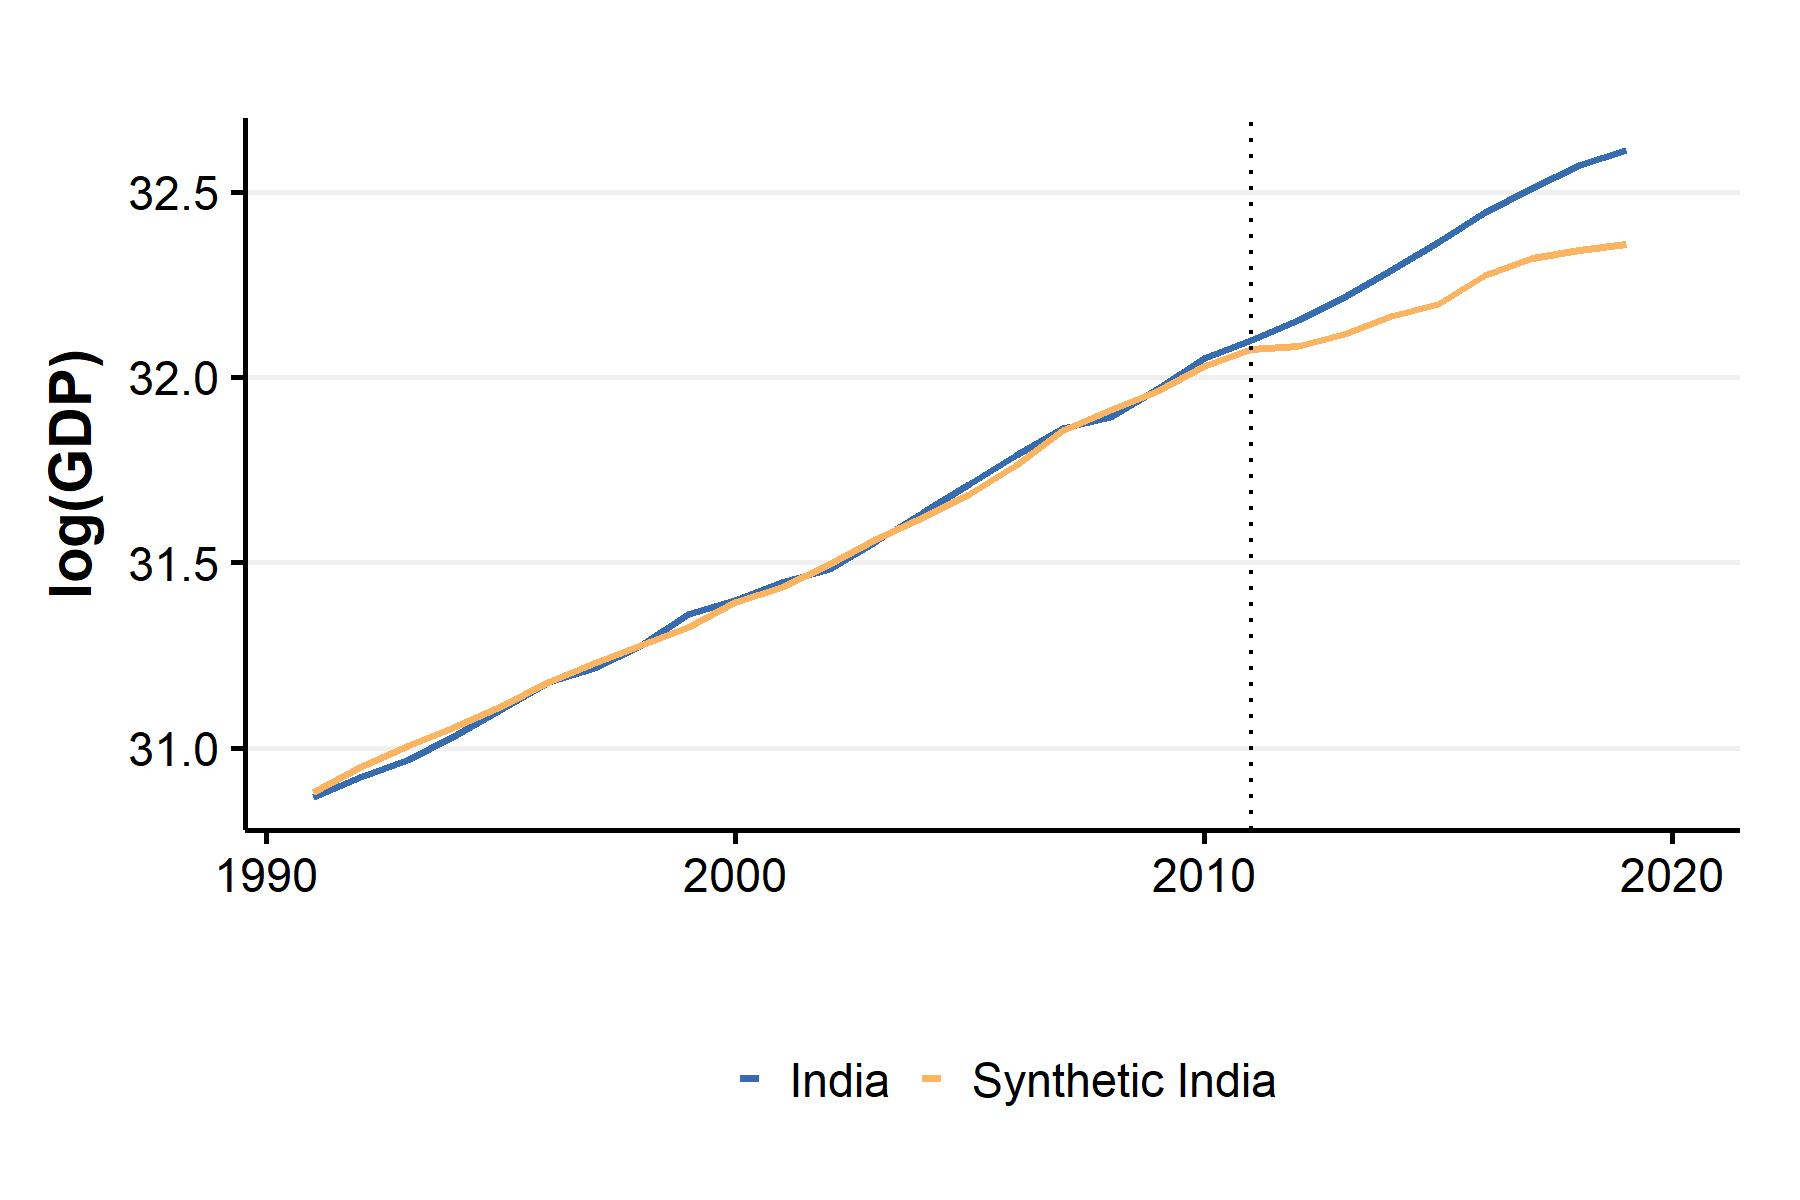
\includegraphics[width=1\linewidth]{figure/indiasynth} 

 }

 \caption{Evolution of Log GDP for India and Synthetic India (SCM)}\label{fig:indsyn}
 \end{figure}
 Figure \ref{fig:indsyn} shows the trend of log GDP for India and the estimated counter factual over the period 1991 - 2019. The counter factual tracks the actual log GDP trend very closely pre - 2011, and starts diverging from the actual trend post - 2011. Given the assumptions of the SCM, the synthetic control is representative of how India's GDP would have evolved in the absence of the change in measurement methodology.
 \begin{figure}

 {\centering 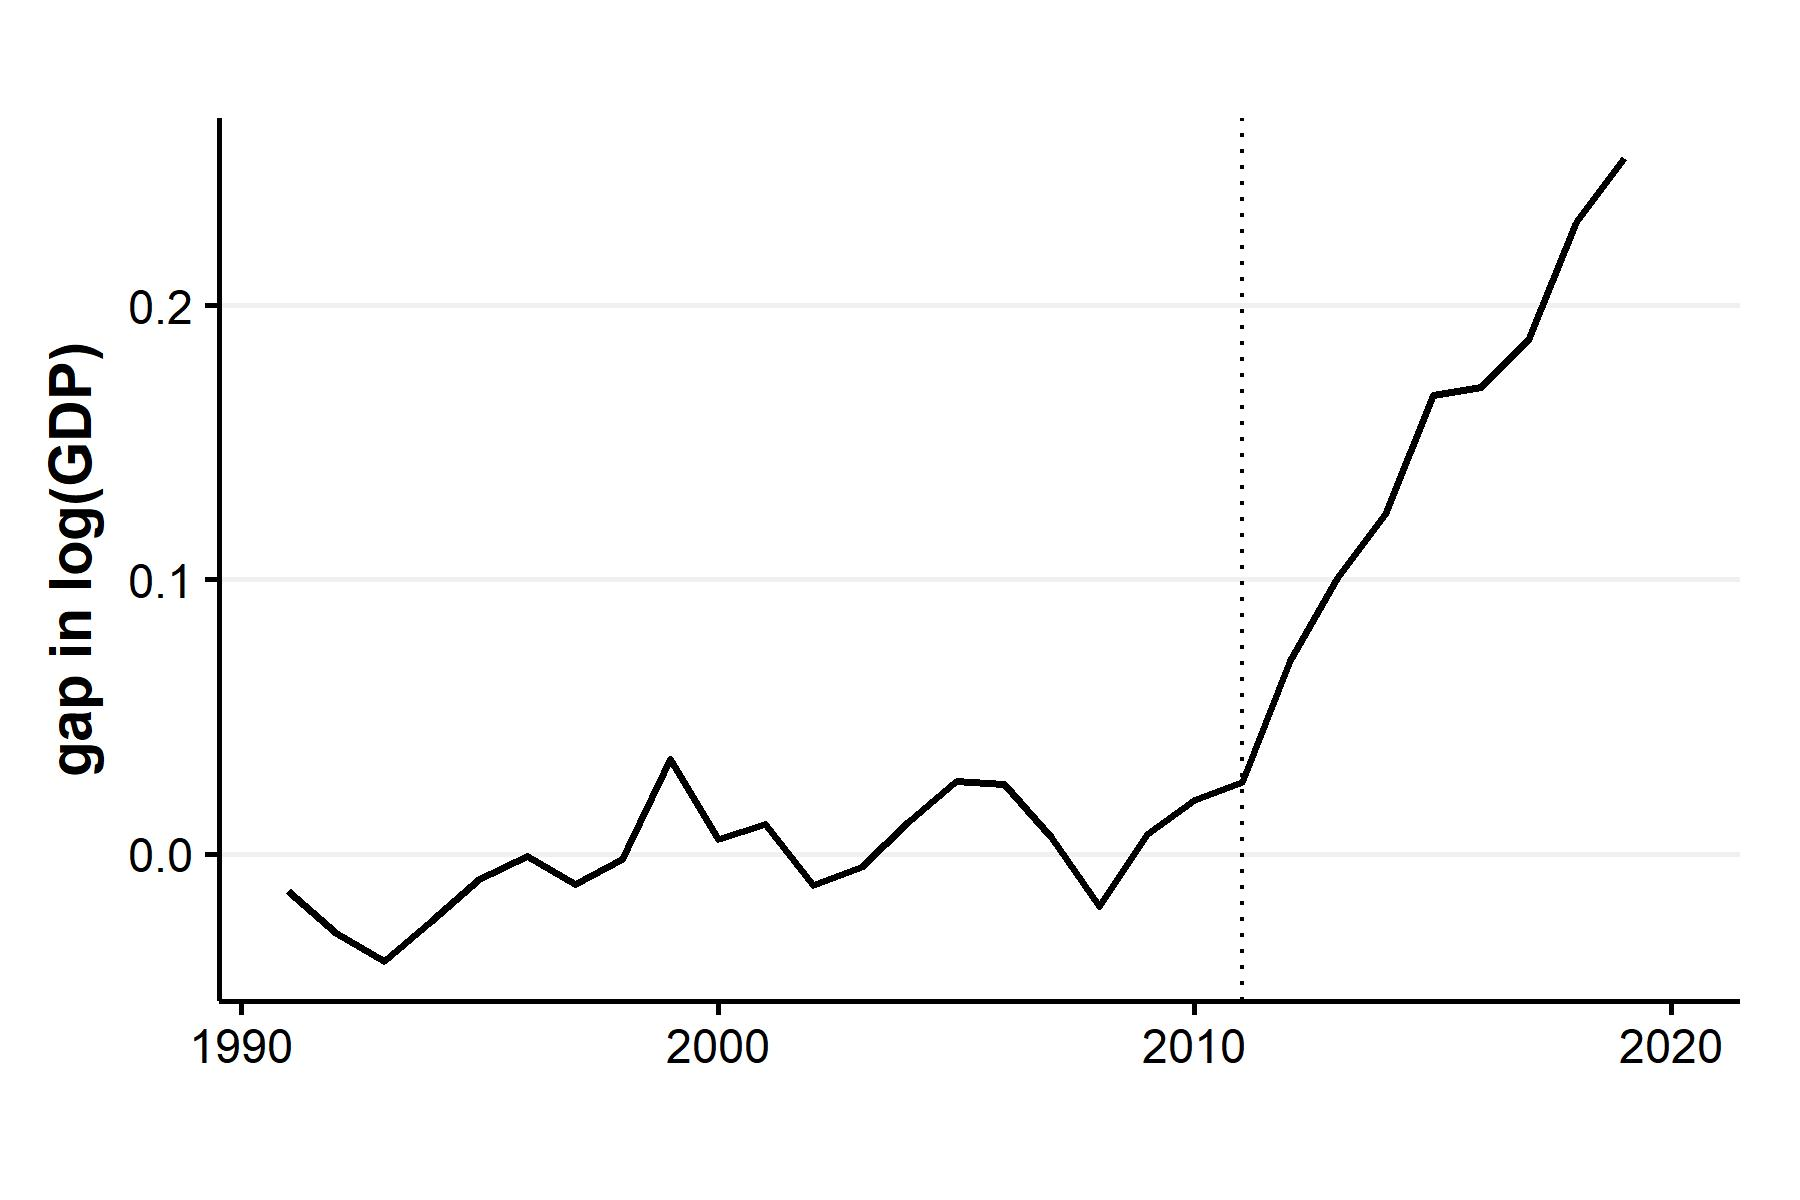
\includegraphics[width=1\linewidth]{figure/indiasynthgap} 

 }

 \caption{Log GDP gap between India and Synthetic India (SCM)}\label{fig:indsyngap}
 \end{figure}
 The same result is shown in a different way in Figure \ref{fig:indsyngap}. This plots the difference between the log GDP trends for actual and synthetic India. As evident from Figure \ref{fig:indiasyn}, the difference remains close to zero pre - treatment, and then increases steadily post - 2011, reaching close to 0.25 log points.
 \linebreak
 \begin{figure}

 {\centering 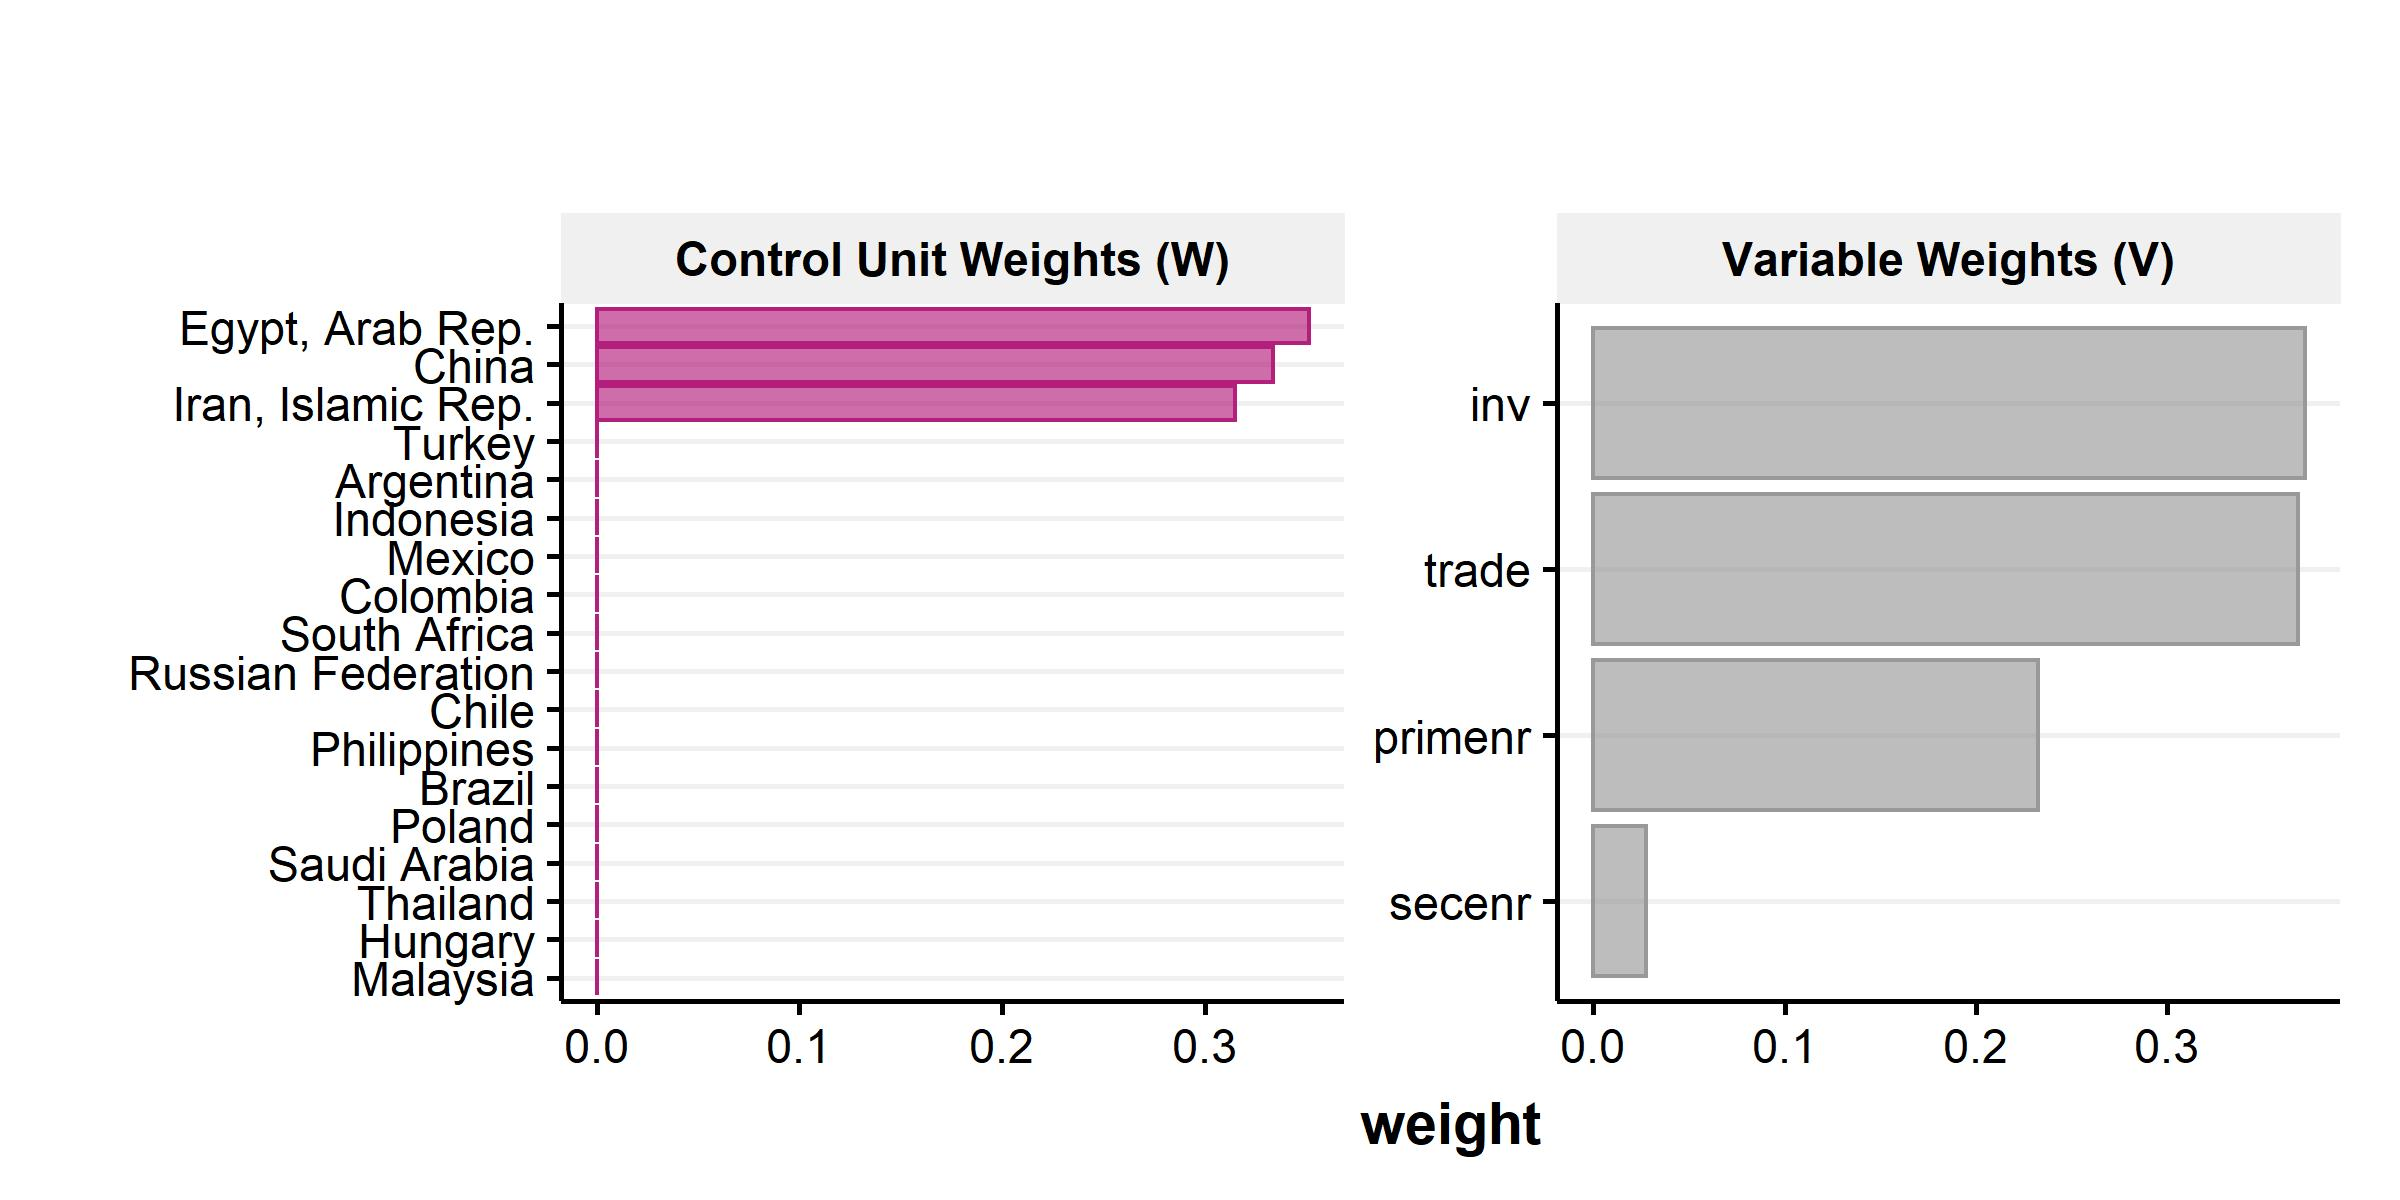
\includegraphics[width=1\linewidth]{figure/weights} 

 }

 \caption{Variable weights and country weights for synthetic India}\label{fig:weights}
 \end{figure}
 Which countries is synthetic India composed of? Figure \ref{fig:weights} shows the optimal country weights, as well as the weights assigned to each predictor. From the left panel, it is clear that synthetic India is composed of Egypt, China and Iran, with each contributing about one -thirds to the total weights. The other countries contribute xlose to nothing. This sparse distribution of weights is a result of the restriction of positive weights summing to one - this prevents extrapolation, and assigns the weights such that the synthetic control lies within the convex hull. The right panel shows the contributions of the predictors: Investment and trade contribute a large share (around 70\%), followed by primary enrollment.
 \linebreak

 I now present the results of the counter factual estimates generated by the GSCM below. Three specifications were run: without covariates, with economic covariates (trade and investment) only, and with all covariates.
 \begin{figure}

 {\centering 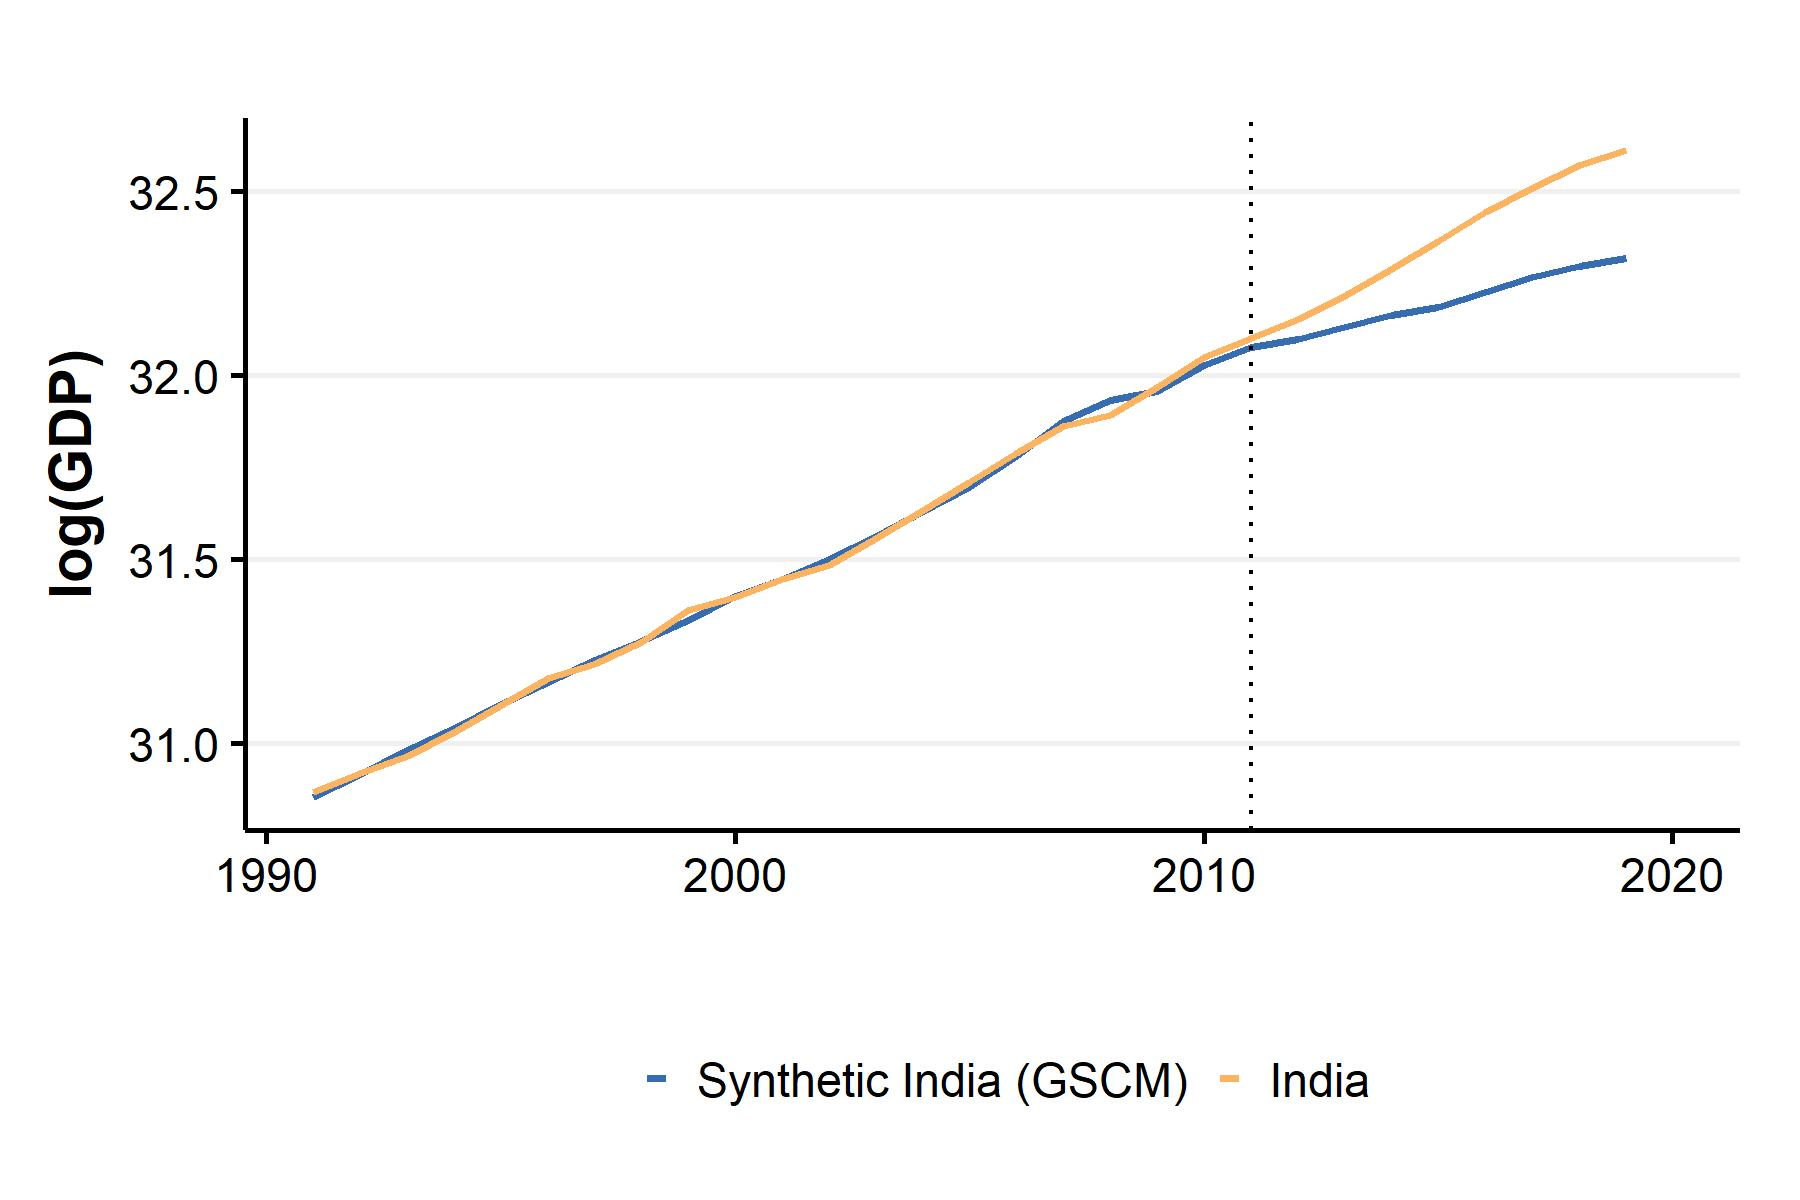
\includegraphics[width=1\linewidth]{figure/indiagsynth} 

 }

 \caption{Evolution of Log GDP for India and Synthetic India (GSCM)}\label{fig:indgsyn}
 \end{figure}
 \newpage
 \begin{figure}

 {\centering 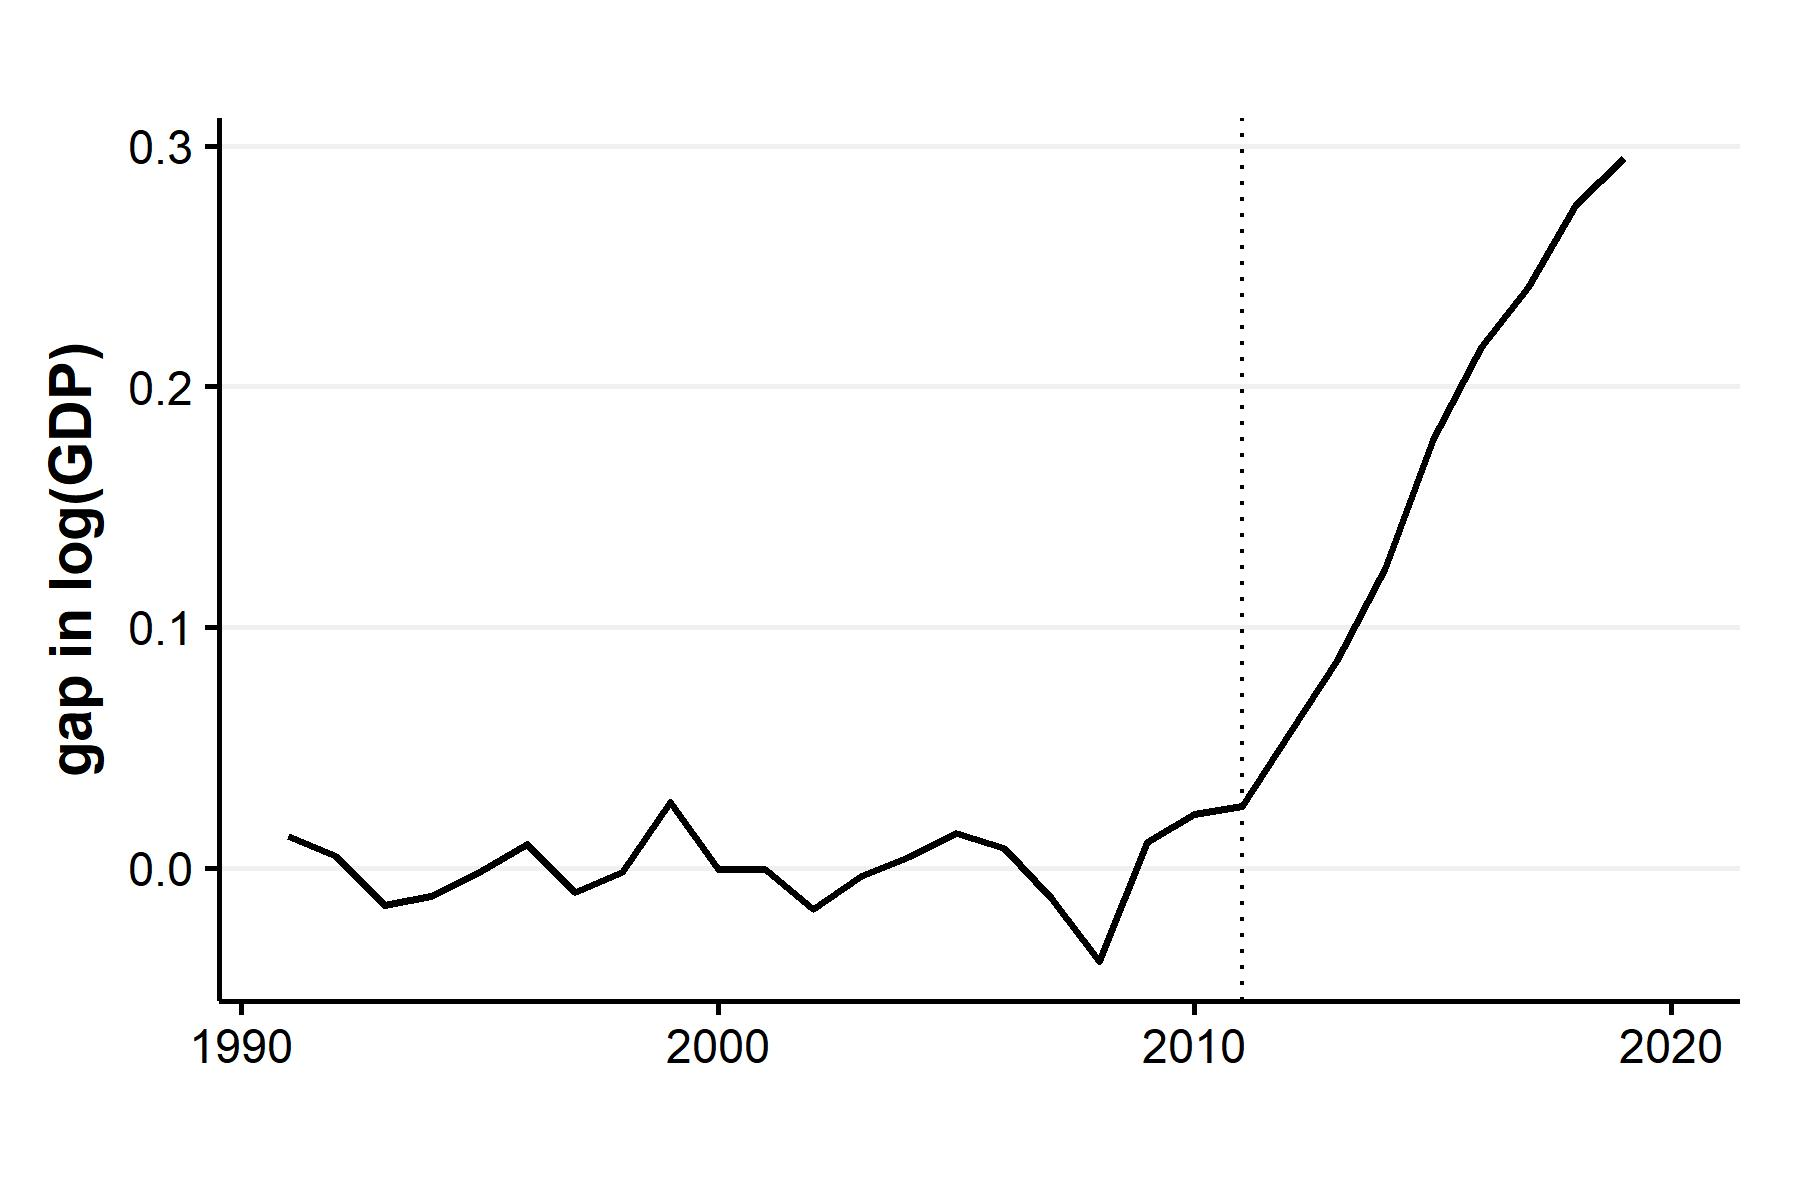
\includegraphics[width=1\linewidth]{figure/indiagsynthgap} 

 }

 \caption{Log GDP gap between India and Synthetic India (GSCM)}\label{fig:indgsyngap}
 \end{figure}
 Figures \ref{fig:indgsyn} and \ref{fig:indgsyngap} show the estimated counterfactual log GDP and actual GDP, and the gap between the two respectively, as measured using the GSCM. As with the SCM, the pre - intervention fit of the counter factual matches the actual trend, and then diverges post - 2011. While the two results look similar, the magnitude of the gap post treatment is different, with the difference exceeding 0.3 log points in case of the GSCM.
 \newpage
 \begin{figure}

 {\centering 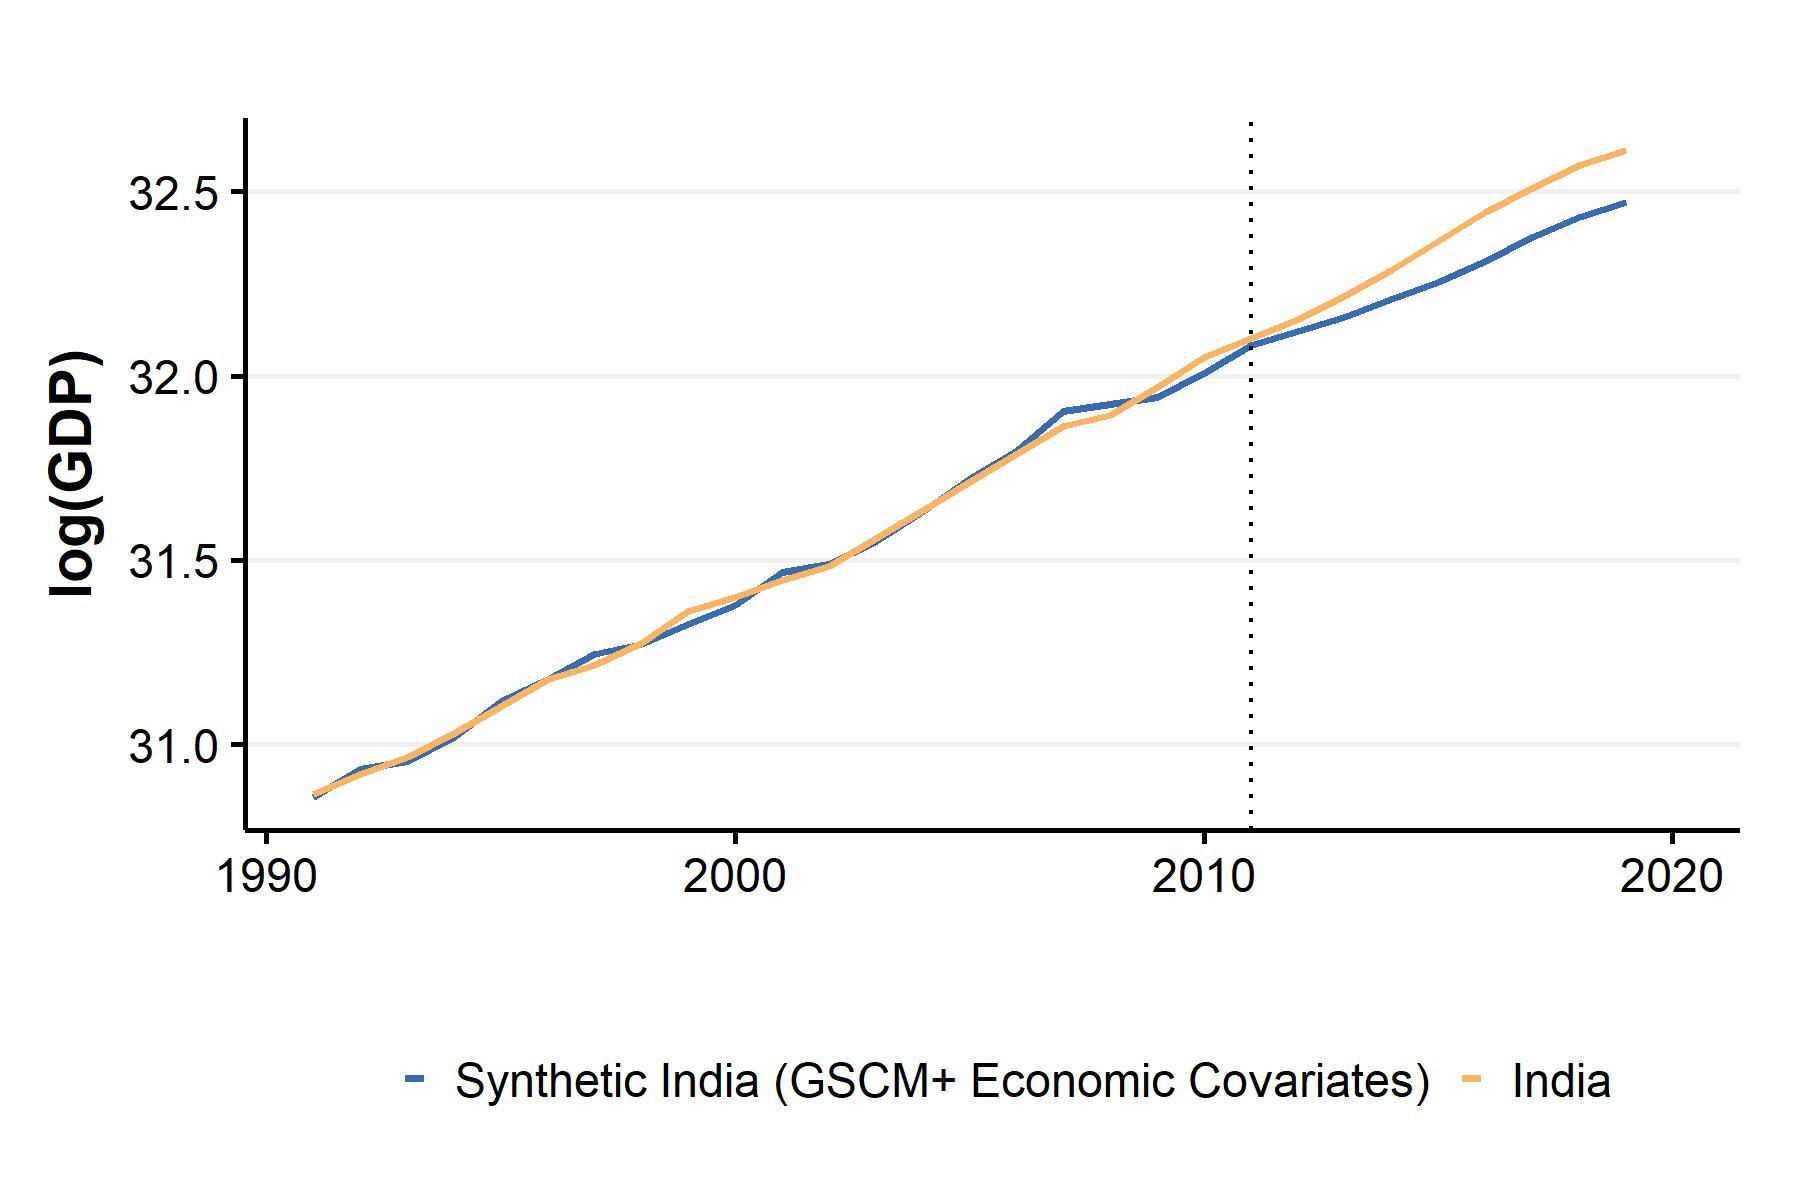
\includegraphics[width=1\linewidth]{figure/indiagsynthc2} 

 }

 \caption{Evolution of Log GDP for India and Synthetic India with economic covariates (GSCM)}\label{fig:indgsync1}
 \end{figure}
 \begin{figure}

 {\centering 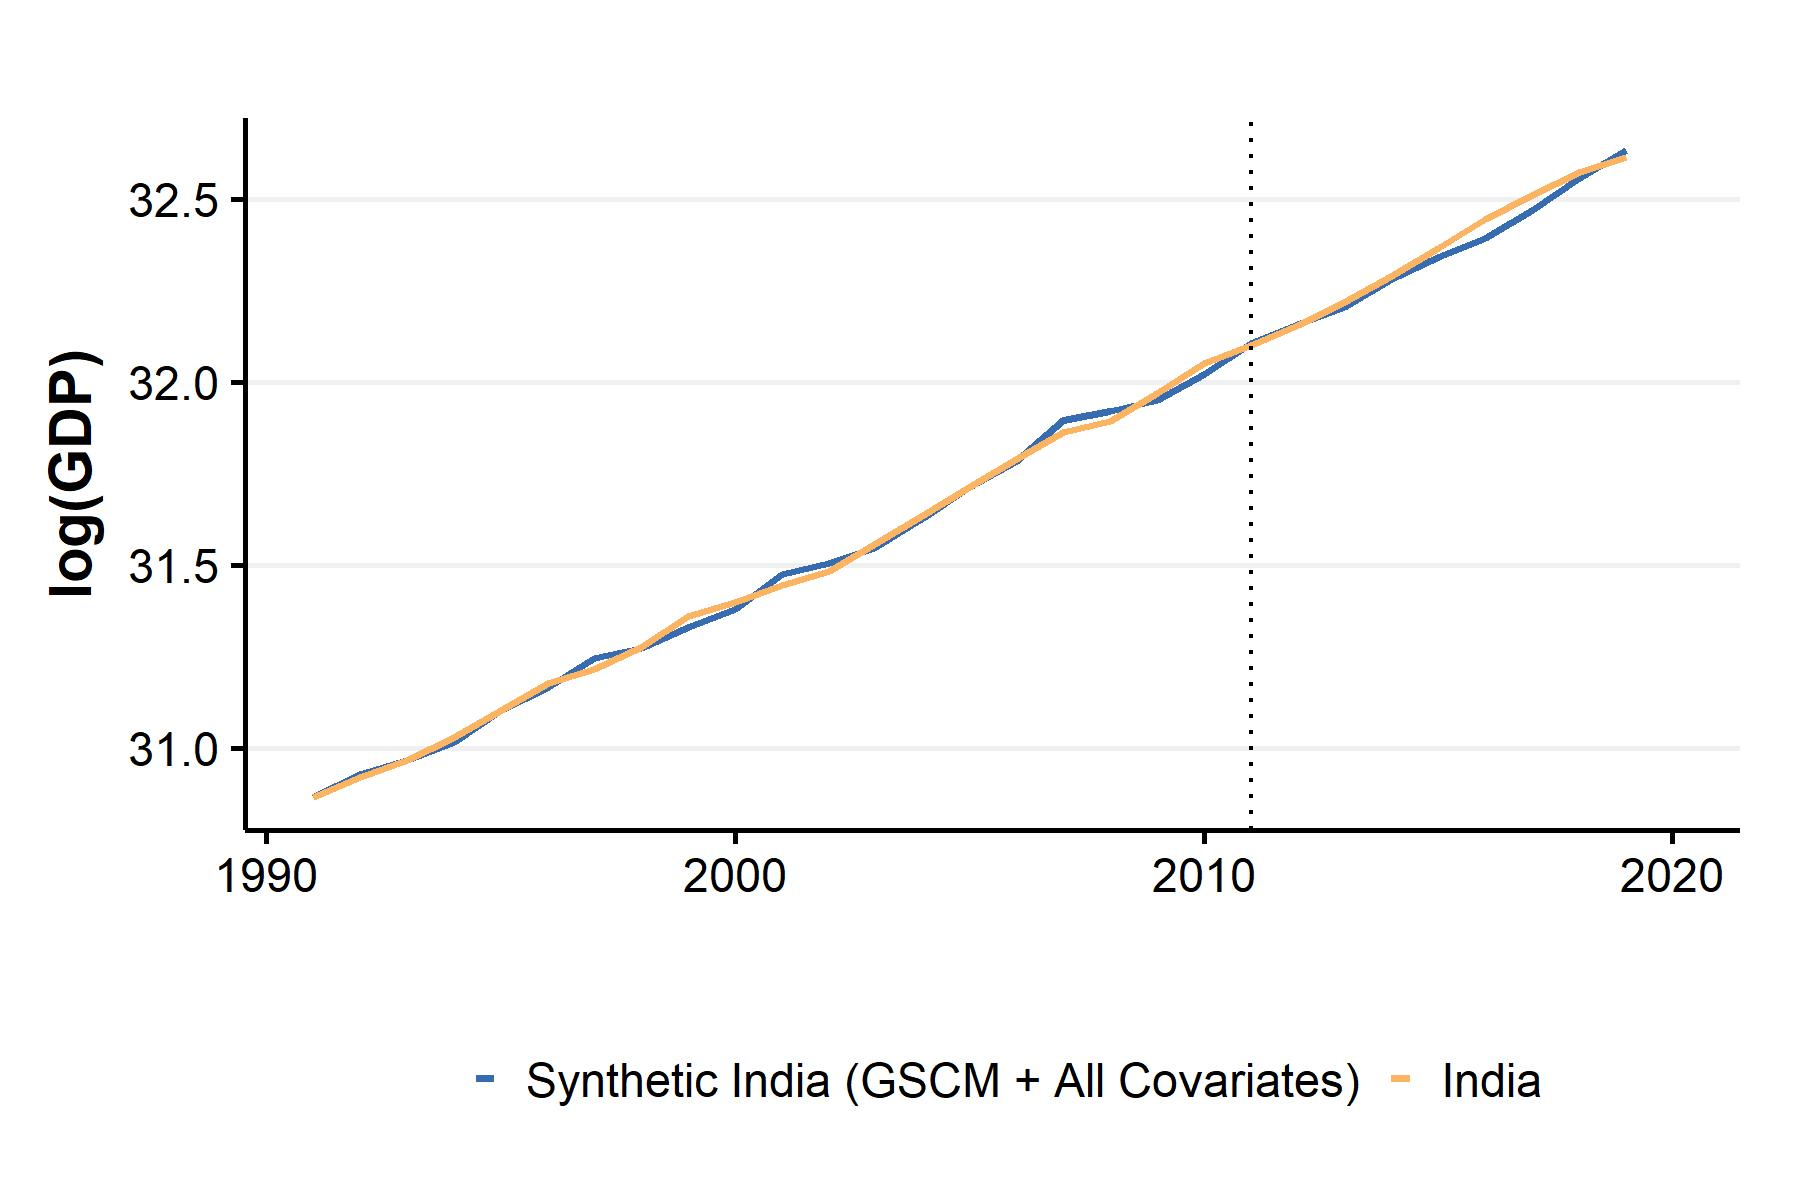
\includegraphics[width=1\linewidth]{figure/indiagsynthc1} 

 }

 \caption{Evolution of Log GDP for India and Synthetic India with all covariates (GSCM)}\label{fig:indgsync2}
 \end{figure}
 Figures \ref{fig:indgsync1} and \ref{fig:indgsync2} show the same results as the images above, but with the inclusion of economic and all covariates respectively. In the first case, the gap post -treatment persists, but at a lower magnitude (around 0.15 log points). In the second, case the post- treatment fit and the pre - treatment fit barely diverge, indicating that the treatment had no impact on India's GDP, when education covariates are included. Hence, the GSCM results are robust to the inclusion of economic covariates, but not to the additional inclusion of education predictors.
 \linebreak

 \newrobustcmd{\B}{\bfseries}
 \begin{table}[h!!]
 \centering
 \begin{tabular}{rrrrr}
 \hline
 Year & SCM & GSCM & GSCM+EC & GSCM+AC\\
 \hline
 2011 & 0.63 & 0.35 & -2.52 & -3.31\\
 \hline
 2012 & 4.45 & 3.06 & 1.38 & -0.03\\
 \hline
 2013 & 3.00 & 3.00 & 2.47 & 1.58\\
 \hline
 2014 & 2.33 & 3.83 & 2.35 & -0.31\\
 \hline
 2015 & 4.34 & 5.38 & 2.96 & 1.54\\
 \hline
 2016 & 0.27 & 3.79 & 2.26 & 2.90\\
 \hline
 2017 & 1.73 & 2.51 & 0.18 & -1.23\\
 \hline
 2018 & 4.29 & 3.45 & 0.89 & -2.32\\
 \hline
 2019 & 2.35 & 1.93 & -0.25 & -3.72\\
 \hline
 \B Avg. & \B 2.6 & \B 3.0 & \B 1.1& \B -0.5\\
 \hline
 \end{tabular}
 \caption{Difference between growth rates (percentage) of actual and synthetic GDP (All specifications)}
 \end{table}
 Table 3.2 shows the difference between the actual and synthetic GDP growth rates for the period 2011 - 2019. The first column shows the growth gap for results estimated using the SCM: except for the year 2016, the difference in growth has exceeded 1.5\% for every year, yielding an average gap of 2.6\% over the whole period. The magnitude is larger for the GSCM estimates without covariates, shown in the second column. Post 2011, the gap has consistently been above 3\%, even crossing 5\% in 2015. The average growth gap in this period broadly matches the findings of Subramanian (\protect\hyperlink{ref-subramanian_indias_2019}{2019}). The inclusion of economic covariates does reduce the average growth gap to 1.1\%, but this is largely due to the period 2017 - 2019; from 2012 - 2017, the average gap exceeded 2\%. The inclusion of education covariates, leads to a significant fluctuation in the growth gap, as seen in the last column. With the gap varying between 2.9\% to -3.7\% over this period, the average growth gap of -0.5\% suggests that there was no significant difference between actual and synthetic India's GDP growth rates.

 \hypertarget{inference-1}{%
 \subsection{Inference}\label{inference-1}}

 The last section presented the results of the estimated counterfactual GDP using two synthetic control techniques. How significant are these findings? In this section, I present the results of the various inference tests used to assess the credibility of the results obtained using the SCM and the GSCM.
 \linebreak

 As discussed in Chapter - 2, Fisher's exact p -values to evaluate the probability of getting the same result had the treatment been randomly assigned to some other country, instead of India. Table - 3.3 presents the p - values below.
 \begin{table}[h!!]
 \centering
 \begin{tabular}{rrr}
 \hline
 Country& Type & p - value\\
 \hline
 India & Treated & \B 0.053\\
 \hline
 Philippines & Donor & 0.105\\
 \hline
 Mexico & Donor & 0.158\\
 \hline
 Brazil & Donor & 0.211\\
 \hline
 Argentina & Donor & 0.263\\
 \hline
 Colombia & Donor & 0.316\\
 \hline
 Chile & Donor & 0.368\\
 \hline
 Indonesia & Donor & 0.421\\
 \hline
 Russian Federation & Donor & 0.474\\
 \hline
 Turkey & Donor & 0.526\\
 \hline
 \end{tabular}
 \caption{Fisher's exact p - values}
 \end{table}
 The p - value for India is 0.053, indicating that there is a 5.3\% probability of getting the same results as those for India. However, the size of the p - value has a lower bound by construction, as it is simply a function of the number of donor units, in this case 1/19. This makes it a unreliably metric for inference.
 \newpage
 \begin{figure}

 {\centering 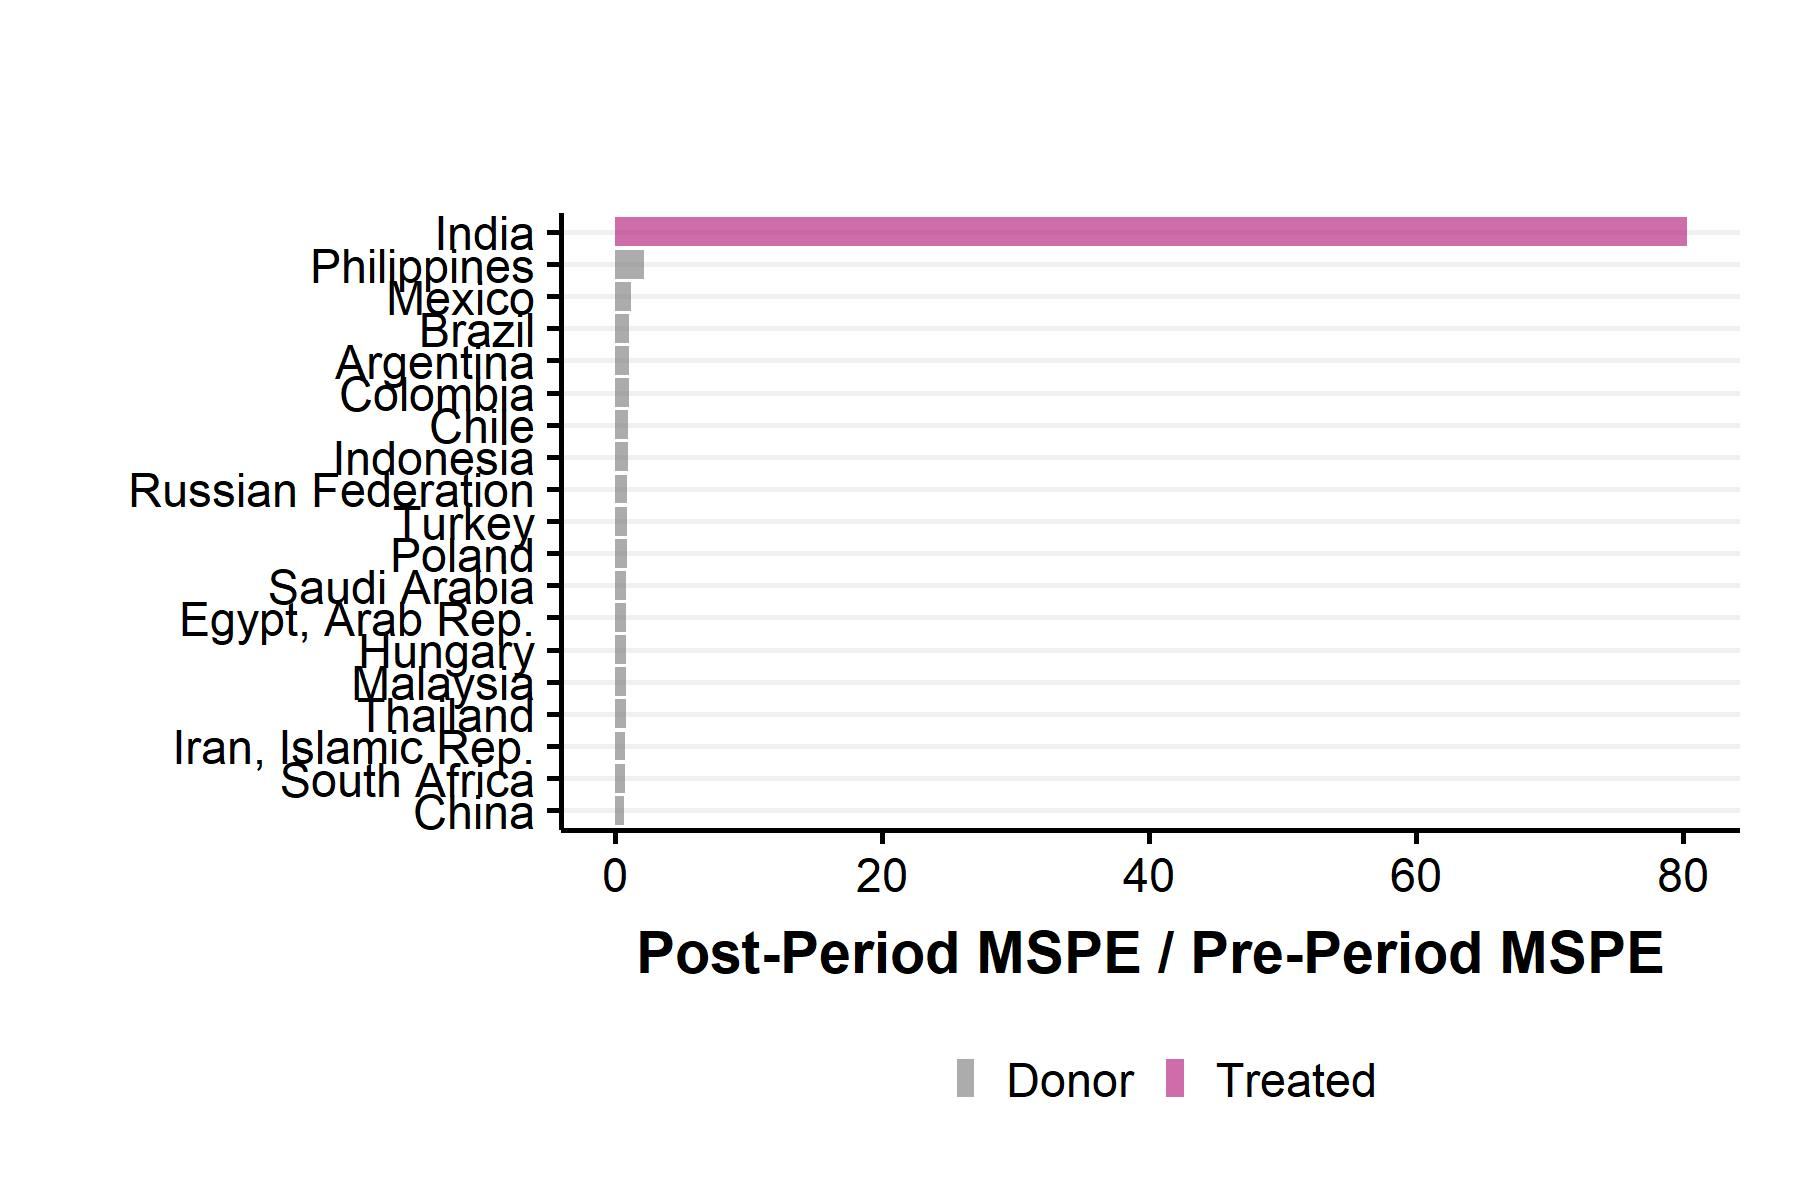
\includegraphics[width=1\linewidth]{figure/msperatio} 

 }

 \caption{Ratio of post and pre - treatment MSPE for India and donor countries}\label{fig:msper}
 \end{figure}
 Figure \ref{fig:msper} shows the ratio of post period and pre - period MSPE. The MSPE is a measure of how close the fit between the actual outcome variable and the synthetic control is. The figure shows the ratio of the MSPE calculated post 2011 and pre 2011 for all donor countries as well as India, serving as a placebo test. The ratio is much higher for India than for the donor pool, indicating that the post treatment fit deviates significantly from the pre - treatment fit to a much larger magnitude relative to other countries. While this is a good starting point to establish the credibility of the synthetic control, it is not a sampling - based statistical test (like a t - test). In the case of the SCM, this is difficult to implement due to absence of a well defined sampling mechanism. Hence, additional robustness tests are required, which are discussed in the next section.
 \begin{table}[h!!]
 \centering
 \begin{tabular}{cccc}
 \hline
 Model & Average ATT & Std. Err. & p - value\\
 \hline
 Baseline GSCM&0.166& 0.256 & 0.516\\
 \hline
 GSCM with economic covariates & 0.094 & 0.139 & 0.499\\
 \hline
 GSCM with all covariates & 0.013 & 0.154 & 0.928\\
 \hline
 \end{tabular}
 \caption{ Average ATT and p - values for GSCM specifications}
 \end{table}
 Table 3.4 shows the average Average Treatment Effect on the Treated, which is simply the mean of the difference between the actual and counterfactual log GDP estimated via GSCM, and the associated p -values. It is important to note that the p - values are calculated in a completely different way from the SCM: rather than a permutation test, uncertainty bounds and variance is estimated using a parametric bootstrap (for details, see Chapter - 2). The results indicate that the mean ATT magnitude falls with the inclusion of covariates and that none of the specifications yield statistically significant results.
 \linebreak

 The lack of significant results could be due to two reasons: one, while the GSCM does allow the inclusion of co -variates with an incomplete panel, the dropping of observations reduces sample size by 50, which is 10\% of the sample. Reduced sample size due to sparse covariate data affects the unbiasedness of the GSCM estimator significantly. Second, Xu (\protect\hyperlink{ref-xu_generalized_2017}{2017}) cautions against a straightforward interpretation of results when the number of donor units is less than 40. Since I use only 19 donor countries, the results are prone to bias.

 \hypertarget{robustness-checks}{%
 \section{Robustness Checks}\label{robustness-checks}}

 I implement two robustness checks:

 \textbf{Backdating}: The treatment is assigned a few years/quarters prior to the actual intervention, and the SCM and GSCM are estimated with the new pre and post treatment periods. The results are robust if:
 \begin{enumerate}
 \def\labelenumi{\alph{enumi}.}
 \item
   The pre - treatment fit does not change between the new and old treatment year, indicating the absence of any anticipation effect.
 \item
   The gap between the synthetic and actual outcome variable of interest starts around the same time as the actual treatment.
   \linebreak
 \end{enumerate}
 I implement the SCM and GSCM by backdating the treatment to the year 2005. This year is chosen so as to allow sufficient pre - intervention time periods (15 years), as atleast 10 years is the minimum recommended for effective implementation of the GSCM.

 \newpage
 \begin{figure}

 {\centering 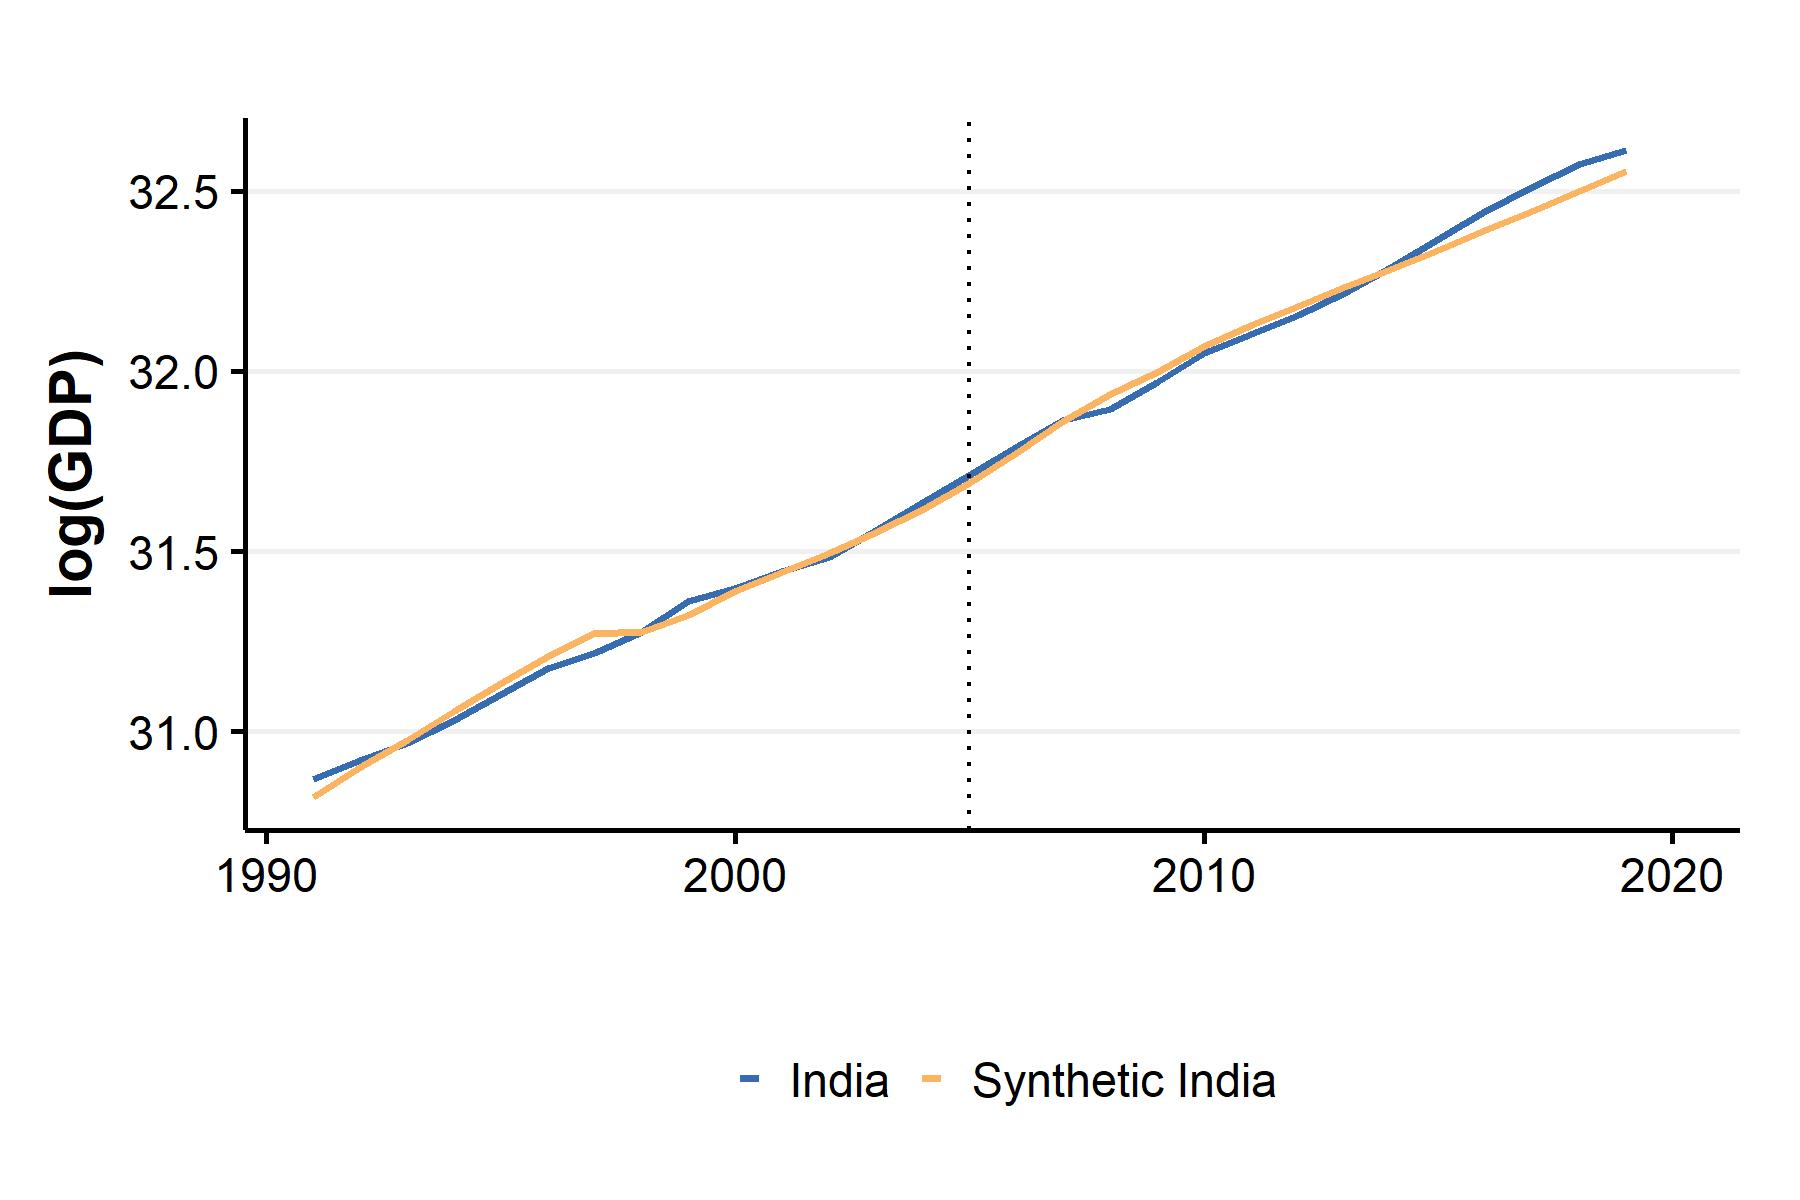
\includegraphics[width=1\linewidth]{figure/indiasynthbd} 

 }

 \caption{Evolution of log GDP for actual and synthetic India with backdated treatment (SCM)}\label{fig:scmbd}
 \end{figure}
 Figure \ref{fig:scmbd} shows the results of backdating implemented using the SCM. Between 2005 and 2011, the synthetic India line closely tracks the actual India line, meeting the first criterion, and ruling out anticipation effects. However, this pattern continues post - 2011 as well, and the first signs of divergence appear only near 2016, five years after the actual treatment, which raises concerns about the credibility of the SCM estimates.
 \newpage
 \begin{figure}

 {\centering 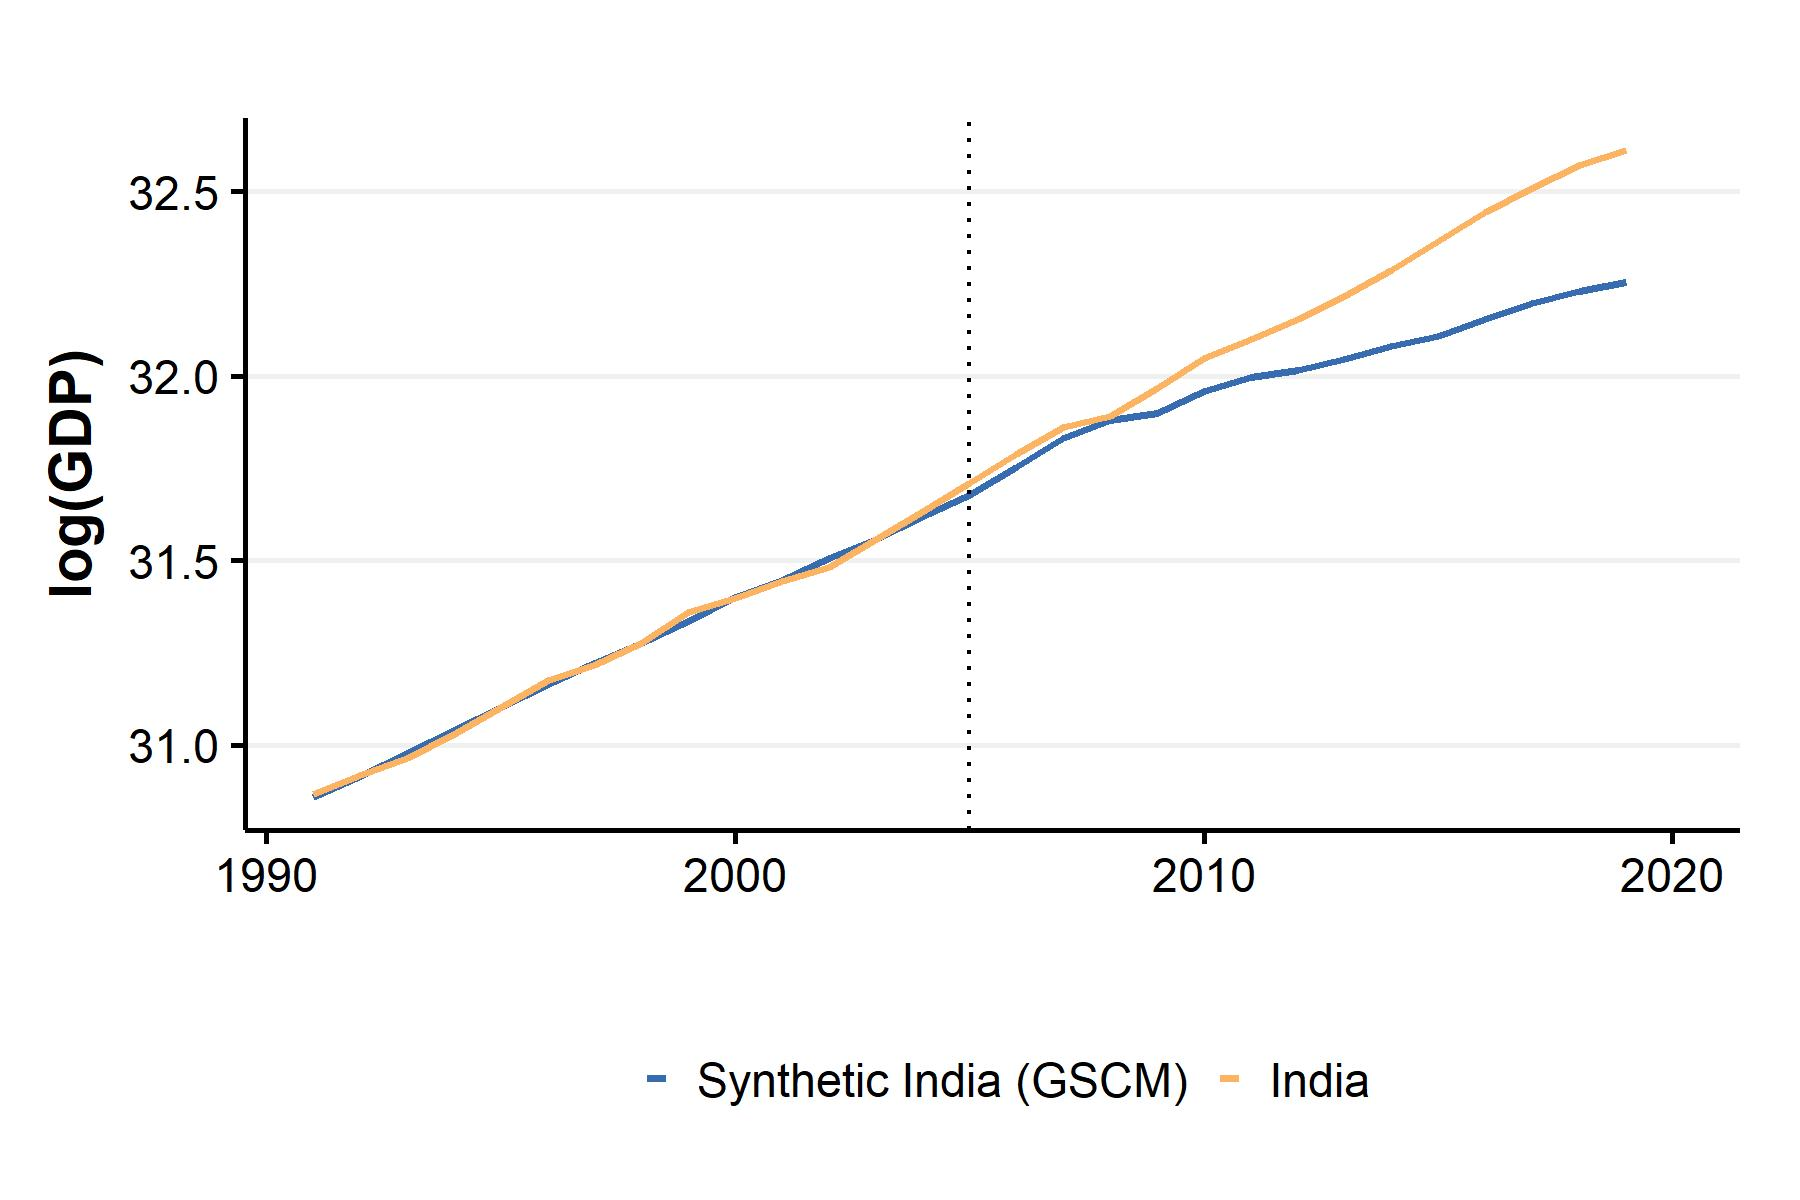
\includegraphics[width=1\linewidth]{figure/indiagsynthbd} 

 }

 \caption{Evolution of log GDP for actual and synthetic India with backdated treatment (GSCM)}\label{fig:gscmbd}
 \end{figure}
 Figure \ref{fig:gscmbd} shows the results of backdating implemented using the GSCM. As previously, there is no gap between the two lines for the period 2005 - 2011. However, the two trends begin to diverge around the actual treatment year, satisfying both conditions for robustness. The backdating procedure indicates that the GSCM estimates are robust relative to SCM.
 \linebreak

 \textbf{Quarterly data}: This robustness check replaces yearly data with quarterly data for the outcome variable. This provides a more granular measure of the GDP, and significantly increases number of observations, attenuating the bias of both estimators. I implement this only for the GSCM, as the SCM requires data for predictors, which was not available on a quarterly basis.
 \linebreak

 The data for quarterly real GDP is taken from the International Monetary Fund's (IMF) International Financial Statistics (IFS) database. The same donor countries were used. The time period is from 1996 Q2 to 2019 Q4, yielding a dataset of 1147 observations.
 \begin{figure}

 {\centering 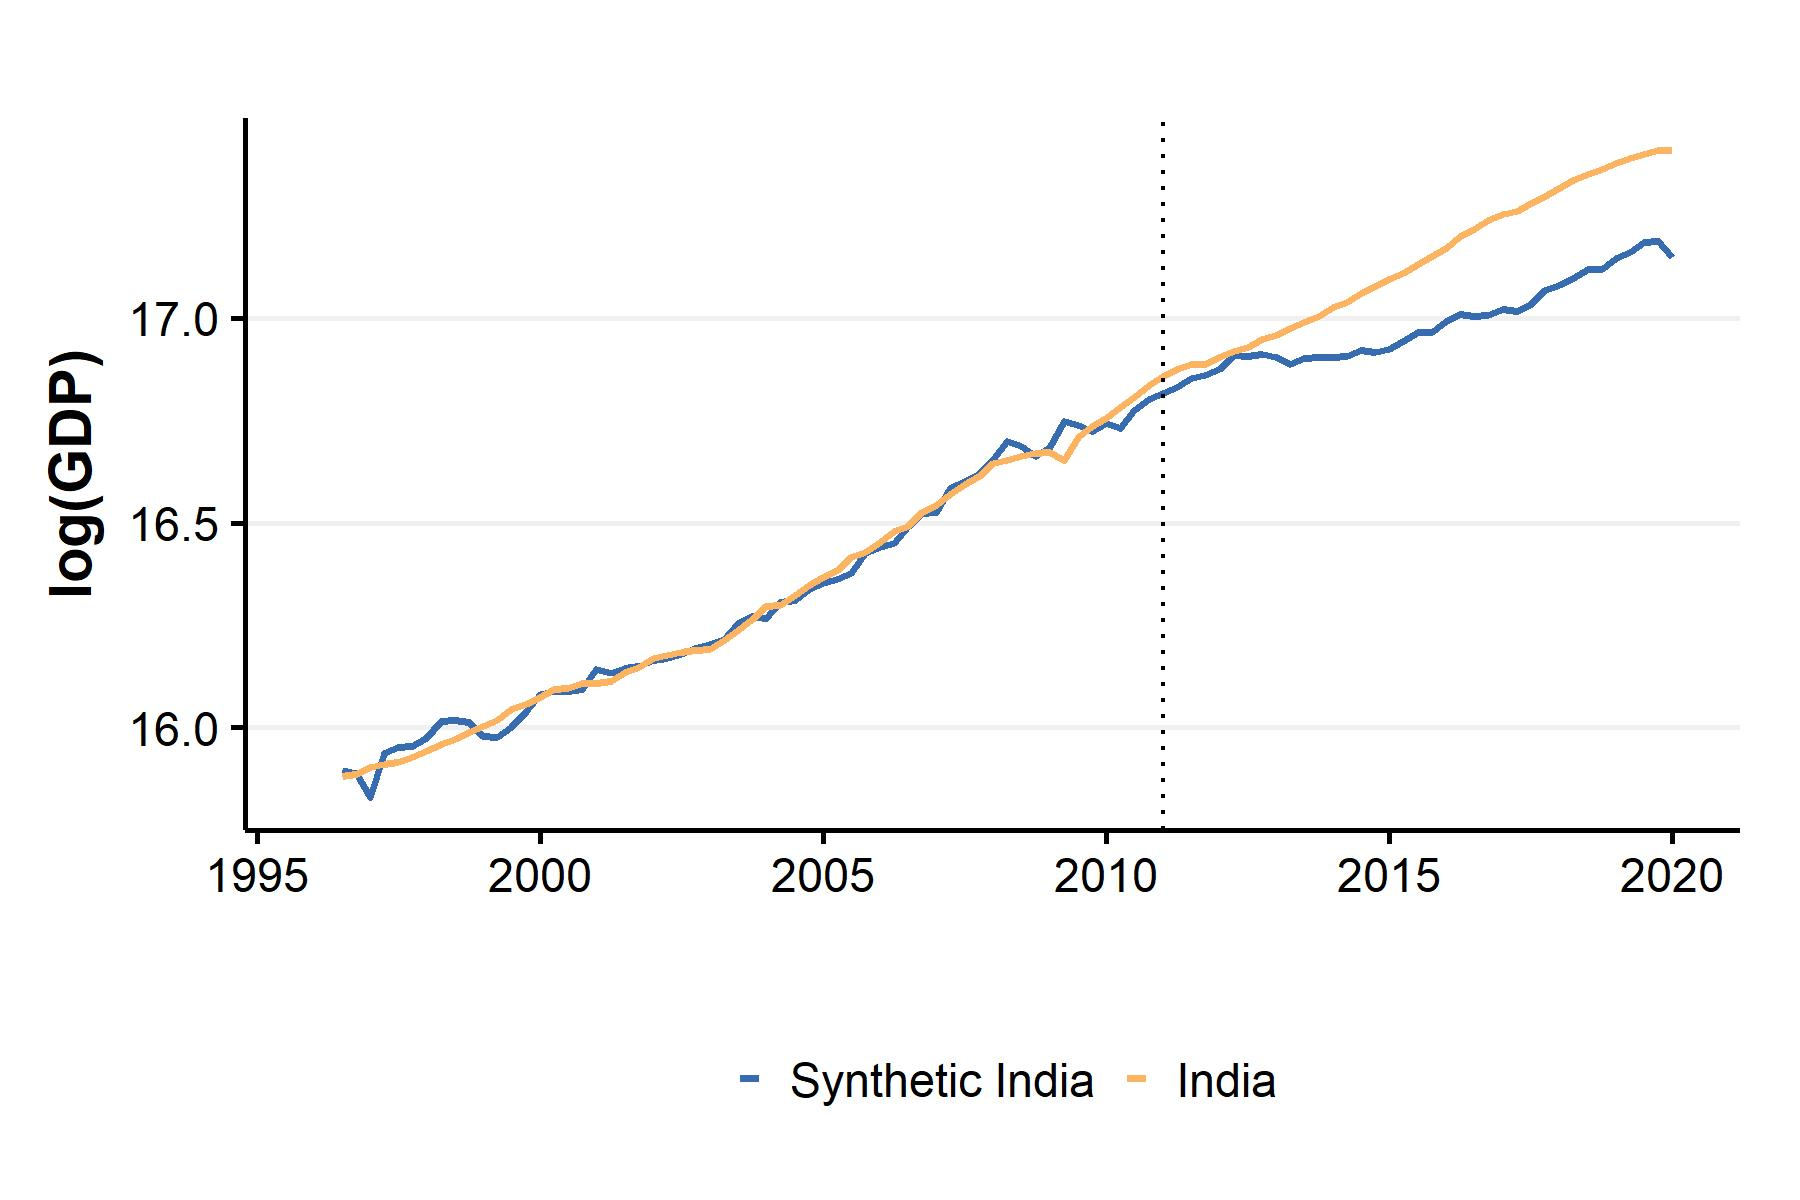
\includegraphics[width=1\linewidth]{figure/indiagsynthqtr} 

 }

 \caption{Evolution of log GDP for actual and synthetic India with quarterly data (GSCM)}\label{fig:gqtr}
 \end{figure}
 Figure \ref{fig:gqtr} shows the results of the above robustness test estimated using the GSCM. The pre - treatment fit remains good prior to 2011. The divergence begins not immediately at 2011 Q1, but almost a year later. However, the overall patterns evolve similar to the SCM and Baseline GSCM results, confirming the robustness of the GSCM results to the use of quarterly data.
 \linebreak

 \hypertarget{discussion-and-conclusion}{%
 \section{Discussion and Conclusion}\label{discussion-and-conclusion}}

 In this chapter, I use the SCM and GSCM to estimate a counterfactual trajectory of India's real GDP. In doing so, I attempt to quantify the extent of conjectured GDP overestimation post - 2011. The SCM results suggest that real GDP growth has been over estimated by 2.6\% on average since the change in base year. However, these results are sensitive to specification, and not fully robust to backdating. The GSCM results, with and without covariates imply that the over-estimation has been between -0.5\% and 3\% on average. The baseline GSCM results are robust to backdating and usage of quarterly data, but statistically insignificant, as are the results with covariates.
 \linebreak

 As discussed before, both the SCM and GSCM perform poorly with low sample size, which is the case in the specifications with predictors, as a number of observations are missing for many countries. Furthermore, a caveat to keep in mind while interpreting these results is that inference for synthetic control and its class of models is an evolving enterprise, and that any results, significant or otherwise need to be interpreted with caution.
 \linebreak

 With regards to the two issues mentioned above, multiple promising avenues have opened up, which serve as a natural extension to this project. The first pertains to development of methods of conformal inference, and exact t - tests by Victor Chernozhukov and co - authors (\protect\hyperlink{ref-chernozhukov_t-test_2021}{Chernozhukov, Wuthrich, et al., 2021}; \protect\hyperlink{ref-chernozhukov_exact_2021}{Chernozhukov, Wüthrich, et al., 2021}). As these methods of inference apply to a large class of causal models, their application to generate uncertainty bounds for SCM results seems like a feasible next step. The second avenue is the development of matrix completion methods for causal models (\protect\hyperlink{ref-athey_matrix_2021}{Athey et al., 2021}), which uses observed control outcome data to impute missing data. Finally, the synthetic difference - in - difference method, which combines the two namesake techniques (\protect\hyperlink{ref-arkhangelsky_synthetic_2021}{Arkhangelsky et al., 2021}) is shown to be more efficient and unbiased relative to both individual methods. The applications of these three novelties form the basis for future research projects regadrding applying the SCM to GDP data.

 \backmatter

 \hypertarget{references}{%
 \chapter*{References}\label{references}}
 \addcontentsline{toc}{chapter}{References}

 \markboth{References}{References}

 \noindent

 \setlength{\parindent}{-0.20in}

 \hypertarget{refs}{}
 \begin{CSLReferences}{1}{0}
 \leavevmode\vadjust pre{\hypertarget{ref-abadie_using_2021}{}}%
 Abadie, A. (2021). Using synthetic controls: Feasibility, data requirements, and methodological aspects. \emph{Journal of Economic Literature}, \emph{59}(2), 391--425. http://doi.org/\href{https://doi.org/10.1257/jel.20191450}{10.1257/jel.20191450}

 \leavevmode\vadjust pre{\hypertarget{ref-abadie_synthetic_2010}{}}%
 Abadie, A., Diamond, A., \& Hainmueller, J. (2010). Synthetic control methods for comparative case studies: Estimating the effect of california's tobacco control program. \emph{Journal of the American Statistical Association}, \emph{105}(490), 493--505. http://doi.org/\href{https://doi.org/10.1198/jasa.2009.ap08746}{10.1198/jasa.2009.ap08746}

 \leavevmode\vadjust pre{\hypertarget{ref-abadie_comparative_2015}{}}%
 Abadie, A., Diamond, A., \& Hainmueller, J. (2015). Comparative politics and the synthetic control method. \emph{American Journal of Political Science}, \emph{59}(2), 495--510. http://doi.org/\href{https://doi.org/10.1111/ajps.12116}{10.1111/ajps.12116}

 \leavevmode\vadjust pre{\hypertarget{ref-abadie_economic_2003}{}}%
 Abadie, A., \& Gardeazabal, J. (2003). The economic costs of conflict: A case study of the basque country. \emph{American Economic Review}, \emph{93}(1), 113--132. http://doi.org/\href{https://doi.org/10.1257/000282803321455188}{10.1257/000282803321455188}

 \leavevmode\vadjust pre{\hypertarget{ref-abadie_penalized_2021}{}}%
 Abadie, A., \& L'Hour, J. (2021). A penalized synthetic control estimator for disaggregated data. \emph{Journal of the American Statistical Association}, \emph{116}(536), 1817--1834. http://doi.org/\href{https://doi.org/10.1080/01621459.2021.1971535}{10.1080/01621459.2021.1971535}

 \leavevmode\vadjust pre{\hypertarget{ref-acemoglu_democracy_2019}{}}%
 Acemoglu, D., Naidu, S., Restrepo, P., \& Robinson, J. A. (2019). Democracy does cause growth. \emph{Journal of Political Economy}, \emph{127}(1), 47--100. http://doi.org/\href{https://doi.org/10.1086/700936}{10.1086/700936}

 \leavevmode\vadjust pre{\hypertarget{ref-amjad_mrsc_2019}{}}%
 Amjad, M., Misra, V., Shah, D., \& Shen, D. (2019). {mRSC}: Multi-dimensional robust synthetic control. \emph{Proceedings of the {ACM} on Measurement and Analysis of Computing Systems}, \emph{3}, 1--27. http://doi.org/\href{https://doi.org/10.1145/3341617.3326152}{10.1145/3341617.3326152}

 \leavevmode\vadjust pre{\hypertarget{ref-amjad_robust_2018}{}}%
 Amjad, M., Shah, D., \& Shen, D. (2018). Robust synthetic control. \emph{Journal of Machine Learning Research}, \emph{19}(22), 1--51. Retrieved from \url{http://jmlr.org/papers/v19/17-777.html}

 \leavevmode\vadjust pre{\hypertarget{ref-arkhangelsky_synthetic_2021}{}}%
 Arkhangelsky, D., Athey, S., Hirshberg, D. A., Imbens, G. W., \& Wager, S. (2021). Synthetic difference-in-differences. \emph{American Economic Review}, \emph{111}(12), 4088--4118. http://doi.org/\href{https://doi.org/10.1257/aer.20190159}{10.1257/aer.20190159}

 \leavevmode\vadjust pre{\hypertarget{ref-aruoba_improving_2013}{}}%
 Aruoba, S. B., Diebold, F. X., Nalewaik, J., Schorfheide, F., \& Song, D. (2013). Improving u.s. {GDP} measurement: A forecast combination perspective. In X. Chen \& N. R. Swanson (Eds.), \emph{Recent advances and future directions in causality, prediction, and specification analysis: Essays in honor of halbert l. White jr} (pp. 1--25). New York, {NY}: Springer. http://doi.org/\href{https://doi.org/10.1007/978-1-4614-1653-1_1}{10.1007/978-1-4614-1653-1\_1}

 \leavevmode\vadjust pre{\hypertarget{ref-aruoba_improving_2016}{}}%
 Aruoba, S. B., Diebold, F. X., Nalewaik, J., Schorfheide, F., \& Song, D. (2016). Improving {GDP} measurement: A measurement-error perspective. \emph{Journal of Econometrics}, \emph{191}(2), 384--397. http://doi.org/\href{https://doi.org/10.1016/j.jeconom.2015.12.009}{10.1016/j.jeconom.2015.12.009}

 \leavevmode\vadjust pre{\hypertarget{ref-athey_matrix_2021}{}}%
 Athey, S., Bayati, M., Doudchenko, N., Imbens, G., \& Khosravi, K. (2021). Matrix completion methods for causal panel data models. \emph{Journal of the American Statistical Association}, \emph{116}(536), 1716--1730. http://doi.org/\href{https://doi.org/10.1080/01621459.2021.1891924}{10.1080/01621459.2021.1891924}

 \leavevmode\vadjust pre{\hypertarget{ref-athey_state_2017}{}}%
 Athey, S., \& Imbens, G. W. (2017). The state of applied econometrics: Causality and policy evaluation. \emph{Journal of Economic Perspectives}, \emph{31}(2), 3--32. http://doi.org/\href{https://doi.org/10.1257/jep.31.2.3}{10.1257/jep.31.2.3}

 \leavevmode\vadjust pre{\hypertarget{ref-bai_panel_2009}{}}%
 Bai, J. (2009). Panel data models with interactive fixed effects. \emph{Econometrica}, \emph{77}(4), 1229--1279. http://doi.org/\href{https://doi.org/10.3982/ECTA6135}{10.3982/ECTA6135}

 \leavevmode\vadjust pre{\hypertarget{ref-becker_estimating_2017}{}}%
 Becker, M., \& Klößner, S. (2017). Estimating the economic costs of organized crime by synthetic control methods. \emph{Journal of Applied Econometrics}, \emph{32}(7), 1367--1369. http://doi.org/\href{https://doi.org/10.1002/jae.2572}{10.1002/jae.2572}

 \leavevmode\vadjust pre{\hypertarget{ref-ben-michael_augmented_2021}{}}%
 Ben-Michael, E., Feller, A., \& Rothstein, J. (2021). The augmented synthetic control method. \emph{Journal of the American Statistical Association}, \emph{116}(536), 1789--1803. http://doi.org/\href{https://doi.org/10.1080/01621459.2021.1929245}{10.1080/01621459.2021.1929245}

 \leavevmode\vadjust pre{\hypertarget{ref-billmeier_assessing_2013}{}}%
 Billmeier, A., \& Nannicini, T. (2013). Assessing economic liberalization episodes: A synthetic control approach. \emph{The Review of Economics and Statistics}, \emph{95}(3), 983--1001. Retrieved from \url{https://econpapers.repec.org/article/tprrestat/v_3a95_3ay_3a2013_3ai_3a3_3ap_3a983-1001.htm}

 \leavevmode\vadjust pre{\hypertarget{ref-card_impact_1990}{}}%
 Card, D. (1990). The impact of the mariel boatlift on the miami labor market. \emph{{ILR} Review}, \emph{43}(2), 245--257. http://doi.org/\href{https://doi.org/10.1177/001979399004300205}{10.1177/001979399004300205}

 \leavevmode\vadjust pre{\hypertarget{ref-card_minimum_1994}{}}%
 Card, D., \& Krueger, A. B. (1994). Minimum wages and employment: A case study of the fast-food industry in new jersey and pennsylvania. \emph{American Economic Review}, \emph{84}(4), 772--793. Retrieved from \url{https://ideas.repec.org/a/aea/aecrev/v84y1994i4p772-93.html}

 \leavevmode\vadjust pre{\hypertarget{ref-chang_measurement_2018}{}}%
 Chang, A. C., \& Li, P. (2018). Measurement error in macroeconomic data and economics research: Data revisions, gross domestic product, and gross domestic income. \emph{Economic Inquiry}, \emph{56}(3), 1846--1869. http://doi.org/\href{https://doi.org/10.1111/ecin.12567}{10.1111/ecin.12567}

 \leavevmode\vadjust pre{\hypertarget{ref-chernozhukov_t-test_2021}{}}%
 Chernozhukov, V., Wuthrich, K., \& Zhu, Y. (2021). \emph{A \$t\$-test for synthetic controls} (No. {arXiv}:1812.10820). {arXiv}. Retrieved from \url{http://arxiv.org/abs/1812.10820}

 \leavevmode\vadjust pre{\hypertarget{ref-chernozhukov_exact_2021}{}}%
 Chernozhukov, V., Wüthrich, K., \& Zhu, Y. (2021). An exact and robust conformal inference method for counterfactual and synthetic controls. \emph{Journal of the American Statistical Association}, \emph{116}(536), 1849--1864. http://doi.org/\href{https://doi.org/10.1080/01621459.2021.1920957}{10.1080/01621459.2021.1920957}

 \leavevmode\vadjust pre{\hypertarget{ref-cso_no_2015}{}}%
 CSO. (2015). No room for doubts on new {GDP} numbers. \emph{Economic and Political Weekly}, \emph{50}(16), 7--8. Retrieved from \url{https://www.epw.in/journal/2015/16/discussion/no-room-doubts-new-gdp-numbers.html}

 \leavevmode\vadjust pre{\hypertarget{ref-cunningham_causal_2021}{}}%
 Cunningham, S. (2021). \emph{Causal inference; the mixtape} (1st ed.). Yale University Press. Retrieved from \url{https://yalebooks.yale.edu/9780300251685/causal-inference}

 \leavevmode\vadjust pre{\hypertarget{ref-doudchenko_balancing_2016}{}}%
 Doudchenko, N., \& Imbens, G. W. (2016). \emph{Balancing, regression, difference-in-differences and synthetic control methods: A synthesis} (Working Paper No. 22791). National Bureau of Economic Research. Retrieved from \url{https://www.nber.org/papers/w22791}

 \leavevmode\vadjust pre{\hypertarget{ref-dube_minimum_2010}{}}%
 Dube, A., Lester, T. W., \& Reich, M. (2010). Minimum wage effects acrss state borders: Estimates using contiguous counties. \emph{The Review of Economics and Statistics}, \emph{92}(4), 945--964. Retrieved from \url{https://www.jstor.org/stable/40985804}

 \leavevmode\vadjust pre{\hypertarget{ref-ferman_synthetic_2021}{}}%
 Ferman, B., \& Pinto, C. (2021). Synthetic controls with imperfect pretreatment fit. \emph{Quantitative Economics}, \emph{12}(4), 1197--1221. http://doi.org/\href{https://doi.org/10.3982/QE1596}{10.3982/QE1596}

 \leavevmode\vadjust pre{\hypertarget{ref-ferman_cherry_2020}{}}%
 Ferman, B., Pinto, C., \& Possebom, V. (2020). Cherry picking with synthetic controls. \emph{Journal of Policy Analysis and Management}, \emph{39}(2), 510--532. http://doi.org/\href{https://doi.org/10.1002/pam.22206}{10.1002/pam.22206}

 \leavevmode\vadjust pre{\hypertarget{ref-hahn_synthetic_2017}{}}%
 Hahn, J., \& Shi, R. (2017). Synthetic control and inference. \emph{Econometrics}, \emph{5}(4), 1--12. Retrieved from \url{https://econpapers.repec.org/article/gamjecnmx/v_3a5_3ay_3a2017_3ai_3a4_3ap_3a52-_3ad_3a120610.htm}

 \leavevmode\vadjust pre{\hypertarget{ref-jacobs_can_2022}{}}%
 Jacobs, J. P. A. M., Sarferaz, S., Sturm, J.-E., \& Norden, S. van. (2022). Can {GDP} measurement be further improved? Data revision and reconciliation. \emph{Journal of Business \& Economic Statistics}, \emph{40}(1), 423--431. http://doi.org/\href{https://doi.org/10.1080/07350015.2020.1831928}{10.1080/07350015.2020.1831928}

 \leavevmode\vadjust pre{\hypertarget{ref-james_introduction_2021}{}}%
 James, G., Witten, D., Hastie, T., \& Tibshirani, R. (2021). \emph{An introduction to statistical learning} (2nd ed.). {NY}: Springer New York. Retrieved from \url{https://link.springer.com/book/10.1007/978-1-0716-1418-1}

 \leavevmode\vadjust pre{\hypertarget{ref-klosner_comparative_2018}{}}%
 Klößner, S., Kaul, A., Pfeifer, G., \& Schieler, M. (2018). Comparative politics and the synthetic control method revisited: A note on abadie et al. (2015). \emph{Swiss Journal of Economics and Statistics}, \emph{154}(1), 11. http://doi.org/\href{https://doi.org/10.1186/s41937-017-0004-9}{10.1186/s41937-017-0004-9}

 \leavevmode\vadjust pre{\hypertarget{ref-kuosmanen_design_2021}{}}%
 Kuosmanen, T., Zhou, X., Eskelinen, J., \& Malo, P. (2021). \emph{Design flaw of the synthetic control method} (No. 106328). University Library of Munich, Germany. Retrieved from \url{https://ideas.repec.org/p/pra/mprapa/106328.html}

 \leavevmode\vadjust pre{\hypertarget{ref-mankiw_are_1984}{}}%
 Mankiw, N. G., Runkle, D. E., \& Shapiro, M. D. (1984). Are preliminary announcements of the money stock rational forecasts? \emph{Journal of Monetary Economics}, \emph{14}(1), 15--27. http://doi.org/\href{https://doi.org/10.1016/0304-3932(84)90024-2}{10.1016/0304-3932(84)90024-2}

 \leavevmode\vadjust pre{\hypertarget{ref-mankiw_news_1986}{}}%
 Mankiw, N. G., \& Shapiro, M. (1986). \emph{News or noise? An analysis of {GNP} revisions} (\{NBER\} Working Paper No. 1939). National Bureau of Economic Research, Inc. Retrieved from \url{https://econpapers.repec.org/paper/nbrnberwo/1939.htm}

 \leavevmode\vadjust pre{\hypertarget{ref-mayberry_economic_2022}{}}%
 Mayberry, A. A. (2022). The economic cost of a nuclear weapon: A synthetic control approach. \emph{Defence and Peace Economics}, \emph{0}(0), 1--20. http://doi.org/\href{https://doi.org/10.1080/10242694.2022.2065186}{10.1080/10242694.2022.2065186}

 \leavevmode\vadjust pre{\hypertarget{ref-nagaraj_seeds_2015-1}{}}%
 Nagaraj, R. (2015a). Seeds of doubt on new {GDP} numbers: Private corporate sector overestimated?, \emph{50}, 14--17.

 \leavevmode\vadjust pre{\hypertarget{ref-nagaraj_seeds_2015}{}}%
 Nagaraj, R. (2015b). Seeds of doubt remain: A reply to {CSO}'s rejoinder. \emph{Economic and Political Weekly}, \emph{50}(18), 64--66. Retrieved from \url{https://www.jstor.org/stable/24481913}

 \leavevmode\vadjust pre{\hypertarget{ref-nagaraj_revisiting_2021}{}}%
 Nagaraj, R. (2021). Revisiting the {GDP} estimation debate. \emph{Economic and Political Weekly}, \emph{56}(45), 10--13. Retrieved from \url{https://www.epw.in/journal/2021/44/commentary/revisiting-gdp-estimation-debate.html}

 \leavevmode\vadjust pre{\hypertarget{ref-singhal_economic_2016}{}}%
 Singhal, S., \& Nilakantan, R. (2016). The economic effects of a counterinsurgency policy in india: A synthetic control analysis. \emph{European Journal of Political Economy}, \emph{45}, 1--17. http://doi.org/\href{https://doi.org/10.1016/j.ejpoleco.2016.08.012}{10.1016/j.ejpoleco.2016.08.012}

 \leavevmode\vadjust pre{\hypertarget{ref-spearman_general_1904}{}}%
 Spearman, C. (1904). "General intelligence," objectively determined and measured. \emph{The American Journal of Psychology}, \emph{15}(2), 201--292. http://doi.org/\href{https://doi.org/10.2307/1412107}{10.2307/1412107}

 \leavevmode\vadjust pre{\hypertarget{ref-subramanian_indias_2019}{}}%
 Subramanian, A. (2019, June). \emph{India's {GDP} mis-estimation: Likelihood, magnitudes, mechanisms, and implications}. \{CID\} Working Paper 354, {CID} Working Paper 354.

 \leavevmode\vadjust pre{\hypertarget{ref-xu_generalized_2017}{}}%
 Xu, Y. (2017). Generalized synthetic control method: Causal inference with interactive fixed effects models. \emph{Political Analysis}, \emph{25}(1), 57--76. http://doi.org/\href{https://doi.org/10.1017/pan.2016.2}{10.1017/pan.2016.2}

 \end{CSLReferences}
	
	% Index?
	
\end{document}
